\documentclass[11pt,a4paper,oneside]{report}

% ---------------- Packages ----------------
\usepackage[T1]{fontenc}
\usepackage[utf8]{inputenc}
\usepackage{lmodern}
\usepackage[margin=2.3cm,headheight=14pt]{geometry}
\usepackage{microtype}
\usepackage{amsmath,amssymb,mathtools,bm}
\usepackage{booktabs,tabularx,longtable,multirow,array}
\usepackage{enumitem}
\usepackage[dvipsnames,table]{xcolor}
\usepackage{tikz}
\usetikzlibrary{arrows.meta,positioning,fit,calc,backgrounds,shapes.geometric,decorations.pathreplacing}
\usepackage[most]{tcolorbox}
\usepackage{caption}
\usepackage{adjustbox}
\usepackage{float}
\usepackage{titlesec}
\usepackage{fancyhdr}
\usepackage[hidelinks]{hyperref}
\usepackage{xurl}

% ---------------- Colours ----------------
\definecolor{acc}{HTML}{1F5E8C}
\definecolor{ink}{HTML}{1F2933}
\definecolor{soft}{HTML}{EEF3F7}
\definecolor{warn}{HTML}{B4561E}
\definecolor{good}{HTML}{2E7D4F}
\definecolor{boxA}{HTML}{DCE9F5}
\definecolor{boxB}{HTML}{F6E7D8}
\definecolor{boxC}{HTML}{E2F0E6}
\definecolor{boxD}{HTML}{EFE4F3}
\definecolor{boxE}{HTML}{F3F3F3}

\hypersetup{colorlinks=true,linkcolor=acc,urlcolor=acc,citecolor=acc}

% ---------------- Layout ----------------
\setlength{\parindent}{0pt}
\setlength{\parskip}{5pt}
\setlist{itemsep=2pt,topsep=3pt}
\titleformat{\chapter}[display]{\normalfont\bfseries\color{ink}}{\large\color{acc}Chapter \thechapter}{4pt}{\LARGE}
\titlespacing*{\chapter}{0pt}{-10pt}{14pt}
\titleformat{\section}{\normalfont\Large\bfseries\color{acc}}{\thesection}{0.6em}{}
\titleformat{\subsection}{\normalfont\large\bfseries\color{ink}}{\thesubsection}{0.6em}{}
\pagestyle{fancy}
\fancyhf{}
\fancyhead[L]{\small\color{gray}Synthetic aneurysm CTA data}
\fancyhead[R]{\small\color{gray}\nouppercase{\leftmark}}
\fancyfoot[C]{\small\thepage}
\renewcommand{\headrulewidth}{0.3pt}
\fancypagestyle{plain}{\fancyhf{}\fancyfoot[C]{\small\thepage}\renewcommand{\headrulewidth}{0pt}}
\captionsetup{font=small,labelfont={bf,color=acc}}

% ---------------- Boxes ----------------
\newtcolorbox{idea}{colback=soft,colframe=acc,boxrule=0.6pt,arc=2pt,left=6pt,right=6pt,top=4pt,bottom=4pt,
  fonttitle=\bfseries,title=In one line}
\newtcolorbox{verdict}[1]{colback=white,colframe=acc,boxrule=0.8pt,arc=2pt,left=6pt,right=6pt,
  fonttitle=\bfseries,title={#1}}
\newtcolorbox{caution}{colback=boxB!60,colframe=warn,boxrule=0.6pt,arc=2pt,left=6pt,right=6pt,
  fonttitle=\bfseries,title=Watch out}
\newtcolorbox{note}{colback=boxE,colframe=gray!60,boxrule=0.4pt,arc=2pt,left=6pt,right=6pt,top=3pt,bottom=3pt}

% ---------------- Maths macros ----------------
\newcommand{\x}{\bm{x}}
\newcommand{\z}{\bm{z}}
\newcommand{\m}{\bm{m}}
\newcommand{\eps}{\bm{\epsilon}}
\newcommand{\E}{\mathbb{E}}
\newcommand{\N}{\mathcal{N}}
\newcommand{\Loss}{\mathcal{L}}
\newcommand{\abar}{\bar{\alpha}}
\newcommand{\enc}{\mathcal{E}}
\newcommand{\dec}{\mathcal{D}}
\newcommand{\R}{\mathbb{R}}
\newcommand{\I}{\bm{I}}
\newcommand{\had}{\odot}
\newcommand{\norm}[1]{\left\lVert #1 \right\rVert}
\DeclareMathOperator{\sg}{sg}
\DeclareMathOperator{\dilate}{dilate}

% ---------------- TikZ styles ----------------
\tikzset{
  blk/.style={draw=ink,rounded corners=2pt,minimum height=9mm,minimum width=20mm,align=center,font=\small,fill=white},
  blkA/.style={blk,fill=boxA},
  blkB/.style={blk,fill=boxB},
  blkC/.style={blk,fill=boxC},
  blkD/.style={blk,fill=boxD},
  blkE/.style={blk,fill=boxE},
  frz/.style={blk,fill=boxE,dashed},
  arr/.style={-{Stealth[length=2.2mm]},thick,draw=ink},
  darr/.style={-{Stealth[length=2.2mm]},thick,dashed,draw=warn},
  lbl/.style={font=\scriptsize,text=ink,align=center},
  grp/.style={draw=acc,rounded corners=4pt,dashed,inner sep=6pt}
}

% Score-card command: #1 name, then six scores 1-5
\newcommand{\stars}[1]{%
  \foreach \i in {1,...,5}{\ifnum\i>#1\textcolor{gray!35}{$\bigstar$}\else\textcolor{acc}{$\bigstar$}\fi}}

\renewcommand{\chaptermark}[1]{\markboth{#1}{}}

\renewcommand{\chaptermark}[1]{\markboth{#1}{}}
\begin{document}
\pagenumbering{roman}

% =================== TITLE ===================
\begin{titlepage}
\centering
\vspace*{3cm}
{\color{acc}\rule{\linewidth}{1pt}}\\[10pt]
{\huge\bfseries\color{ink} Generating Synthetic Aneurysm\\[4pt] CTA Data with Masks\\[4pt] Using Generative Models}\\[10pt]
{\color{acc}\rule{\linewidth}{1pt}}\\[18pt]
{\Large Eight methods. For each: the paper, the maths,\\ and what we do with our dataset.}\\[40pt]
\begin{tabular}{rl}
\textbf{Dataset} & Intracranial aneurysm CTA (Bo et al., \emph{Patterns} 2021)\\
\textbf{Data now} & 99 scan + mask pairs (Tr0001--Tr0099)\\
\textbf{Data planned} & $\approx$1{,}338 scan + mask pairs (full internal set)\\
\textbf{Prepared for} & Charitha\\
\textbf{Date} & November 2026
\end{tabular}
\vfill
{\small Figures are redrawn by us from the cited papers.\\
``(paper)'' = number from the paper. ``(estimate)'' = our rough guess.}
\end{titlepage}

\tableofcontents
\clearpage

% =================== HOW TO READ ===================
\chapter*{How to read this document}
\addcontentsline{toc}{chapter}{How to read this document}

\textbf{Goal.} Make new CTA scans that contain brain aneurysms, \emph{with} an exact mask for each aneurysm. Use them to train better aneurysm segmentation models.

\textbf{How each method chapter is built.} Every method chapter (Chapters~\ref{ch:lefusion}--\ref{ch:spade}) stands on its own and has two parts:

\begin{center}
\begin{tabular}{p{0.42\linewidth}p{0.48\linewidth}}
\toprule
\textbf{Part A -- The paper} & \textbf{Part B -- Our dataset} \\
\midrule
A.1 Idea in simple words & B.1 What data this method needs \\
A.2 Basics you need (maths) & B.2 How we train it (scratch / fine-tune / LoRA) \\
A.3 Architecture (figure) & B.3 Step-by-step pipeline \\
A.4 Maths and loss & B.4 Compute \\
A.5 Input and output & B.5 How to check it worked \\
A.6 Results in the paper & B.6 Risks \\
 & B.7 Rank for our dataset \\
\bottomrule
\end{tabular}
\end{center}

\textbf{Other chapters.}
\begin{itemize}
  \item Chapter~\ref{ch:intro}: our dataset in short.
  \item Chapter~\ref{ch:prep}: common steps that all methods share (split, preprocessing, where to place an aneurysm). Part B of each method says which of these steps it needs.
  \item Chapter~\ref{ch:baseline}: a simple non-AI baseline to compare against.
  \item Chapter~\ref{ch:eval}: one fair test for all methods.
  \item Chapter~\ref{ch:licence}: dataset licence.
  \item Chapter~\ref{ch:summary}: summary, ranking and roadmap.
\end{itemize}

\textbf{The eight methods, in our ranked order.}
\begin{center}
\small
\begin{tabular}{clll}
\toprule
\textbf{Rank} & \textbf{Method} & \textbf{Type} & \textbf{Works on} \\
\midrule
1 & LeFusion & diffusion, fills a mask & small 3D patch \\
2 & DiffTumor & latent diffusion, fills a mask & small 3D patch \\
3 & 3D cGAN (Jin et al.) & GAN, fills a mask & small 3D patch \\
4 & RePaint & diffusion, fills a mask (no extra training) & small 3D patch \\
5 & MAISI / MAISI-v2 + ControlNet & big pretrained model & large 3D region \\
6 & Med-DDPM & diffusion, label map $\rightarrow$ image & 3D region \\
7 & MedGen3D & diffusion, makes mask \emph{and} image & 3D region (2.5D) \\
8 & brainSPADE & label generator + GAN & 2D slices \\
\bottomrule
\end{tabular}
\end{center}

\textbf{Two data cases.}
\begin{itemize}
  \item \textbf{Case A (now):} 99 scans, about 117 aneurysms. Good for testing code only.
  \item \textbf{Case B (planned):} about 1{,}338 scans, about 1{,}489 aneurysms. The ranking assumes this case.
\end{itemize}

\clearpage\pagenumbering{arabic}
% =================== CHAPTER 1 ===================
\chapter{Our dataset in short}\label{ch:intro}

\section{What we have}
Head CT angiography (CTA) from Bo et al.~\cite{bo2021}. In CTA, dye is in the blood, so arteries look bright.

\begin{center}
\begin{tabularx}{\linewidth}{lX}
\toprule
\textbf{Part} & \textbf{Content} \\
\midrule
Scans & 99 now ($\approx$1{,}338 planned); $512\times512\times N$ voxels; values in HU, $-1024$ to $3071$ \\
Internal masks & 1{,}338 (1{,}186 train, 152 test of which 50 have no aneurysm); 1 = aneurysm \\
External masks & 138 from two other hospitals + CSV (age, sex, rupture, number of aneurysms) \\
Voxel size & 0.32--0.70\,mm in-plane; 0.4--1.0\,mm between slices (mostly 0.4\,mm) \\
Aneurysm size & median $\approx$74\,mm$^3$; about 5\,mm across (most between 3 and 11\,mm) \\
\bottomrule
\end{tabularx}
\end{center}

\section{Why this is hard}
\begin{itemize}
  \item \textbf{Very small target.} A 5\,mm aneurysm is only about 11 voxels across.
  \item \textbf{It must sit on a vessel.} A fake aneurysm floating in brain tissue is useless.
  \item \textbf{No normal scans for training.} All training cases have aneurysms.
  \item \textbf{Big 3D files.} One scan can take 500\,MB in memory, so most methods work on small boxes (patches).
\end{itemize}

\section{Two ways to make synthetic data}
\begin{enumerate}
  \item \textbf{Fill a mask in a real scan (inpainting).} Pick a spot on a vessel, give a mask shape, let the model draw an aneurysm inside. The rest of the scan stays real. \emph{(Methods 1--4.)}
  \item \textbf{Make a whole region.} Give a label map (vessels + aneurysm) and generate a full region. \emph{(Methods 5--8.)}
\end{enumerate}
Way 1 needs less data and compute, and keeps most of the scan real. That is why methods 1--4 rank higher.

\section{Symbols used}
\begin{center}
\small
\begin{tabular}{ll}
\toprule
\textbf{Symbol} & \textbf{Meaning} \\
\midrule
$\x$ & a CT patch (normalised HU) \\
$\m$ & aneurysm mask (1 = aneurysm) \\
$\bm v$ & vessel map \\
$\enc,\ \dec$ & encoder, decoder \\
$\z$ & latent code (compressed image) \\
$t,\ T$ & diffusion step, number of steps \\
$\beta_t,\ \alpha_t=1-\beta_t,\ \abar_t=\prod_{s\le t}\alpha_s$ & noise schedule \\
$\eps\sim\N(\bm 0,\I)$ & random Gaussian noise \\
$\eps_\theta$ & network that predicts noise \\
$\had$ & multiply element by element \\
$G,\ D$ & GAN generator, discriminator \\
\bottomrule
\end{tabular}
\end{center}

% =================== CHAPTER 2 ===================
\chapter{Common steps for all methods}\label{ch:prep}

All eight methods need the same groundwork. We describe it once here. Each method's Part~B lists which of these steps it uses.

\begin{figure}[H]
\centering
\begin{adjustbox}{max width=\linewidth}
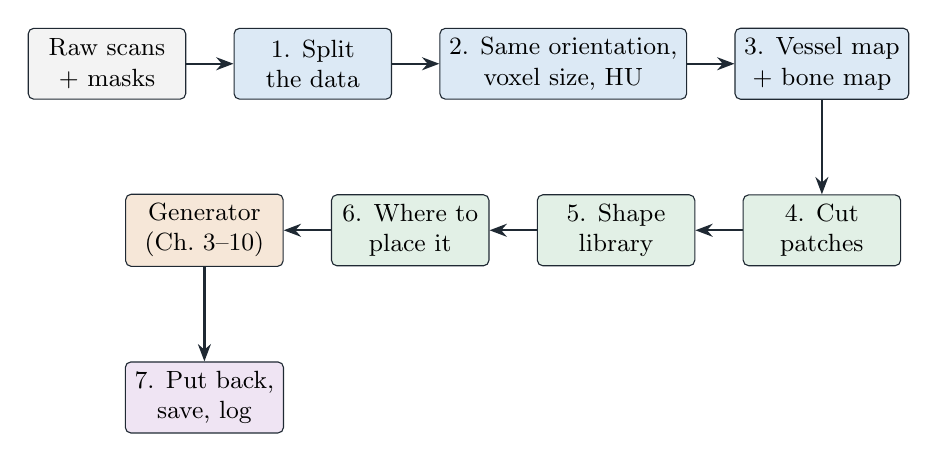
\begin{tikzpicture}[node distance=5mm and 6mm]
\node[blkE] (raw) {Raw scans\\+ masks};
\node[blkA, right=of raw] (split) {1. Split\\the data};
\node[blkA, right=of split] (pre) {2. Same orientation,\\voxel size, HU};
\node[blkA, right=of pre] (ves) {3. Vessel map\\+ bone map};
\node[blkC, below=12mm of ves] (patch) {4. Cut\\patches};
\node[blkC, left=of patch] (shape) {5. Shape\\library};
\node[blkC, left=of shape] (place) {6. Where to\\place it};
\node[blkB, left=of place] (gen) {Generator\\(Ch.\ 3--10)};
\node[blkD, below=12mm of gen] (paste) {7. Put back,\\save, log};
\draw[arr] (raw)--(split); \draw[arr] (split)--(pre); \draw[arr] (pre)--(ves);
\draw[arr] (ves)--(patch); \draw[arr] (patch)--(shape); \draw[arr] (shape)--(place); \draw[arr] (place)--(gen);
\draw[arr] (gen)--(paste);
\end{tikzpicture}
\end{adjustbox}
\caption{Common steps. Only the green ``Generator'' box changes between methods.}
\label{fig:prep}
\end{figure}


\section*{Step 1 -- Split the data first}
\addcontentsline{toc}{section}{Step 1 -- Split the data first}
\begin{center}
\small
\begin{tabular}{lll}
\toprule
\textbf{Set} & \textbf{Cases} & \textbf{Used for} \\
\midrule
Train & $\approx$1{,}000 \texttt{Tr} & training generators and segmenters \\
Validation & $\approx$186 \texttt{Tr} & choosing settings; never seen by generators \\
Test & 152 \texttt{Ts} & final test only \\
External & 138 \texttt{Ext} (needs scans) & final outside test only \\
\bottomrule
\end{tabular}
\end{center}
\begin{caution}
Train generators on the \textbf{train} set only. If they see validation or test scans, results will look better than they really are. In Case A (99 scans) use about 80 for training and 19 for validation.
\end{caution}

\section*{Step 2 -- Make all scans look the same}
\addcontentsline{toc}{section}{Step 2 -- Make all scans look the same}
\begin{enumerate}
  \item \textbf{Same orientation} (RAS) with \texttt{nib.as\_closest\_canonical}. This also fixes Tr0370.
  \item \textbf{Same voxel size}: 0.45\,mm in all directions. Linear interpolation for scans, nearest for masks.
  \item \textbf{Same value range}: keep HU between $-100$ and $900$ and scale to $[-1,1]$:
  \begin{equation}
  \tilde x = 2\cdot\frac{\operatorname{clip}(x,-100,900)+100}{1000} - 1 .
  \end{equation}
  \item \textbf{Clean masks}: delete blobs under 20 voxels (e.g.\ in Tr0734).
\end{enumerate}

\section*{Step 3 -- Vessel map and bone map}
\addcontentsline{toc}{section}{Step 3 -- Vessel map and bone map}
\begin{align}
\text{bone} &= \text{grow}_{2\,\text{mm}}\Big(\text{big blobs of }(x>700\,\text{HU})\Big),\\
\bm v &= (x > 200\,\text{HU})\ \text{and not bone}.
\end{align}
\begin{note}
Near the skull base the carotid artery touches bone and may be removed. Check this area by eye.
\end{note}

\section*{Step 4 -- Cut patches}
\addcontentsline{toc}{section}{Step 4 -- Cut patches}
\begin{center}
\small
\begin{tabular}{llll}
\toprule
\textbf{Patch} & \textbf{Size} & \textbf{How many (Case B)} & \textbf{What is in it} \\
\midrule
Aneurysm patch & $64^3$ ($\approx$29\,mm) & $\approx$1{,}300 & a real aneurysm in the centre \\
Normal vessel patch & $64^3$ & $\approx$5{,}000 & vessel branch, far from aneurysms \\
Region crop & $128^3$--$256^3$ & $\approx$1{,}000 & area around the circle of Willis \\
\bottomrule
\end{tabular}
\end{center}
All patches together are a few GB, so they are easy to upload to a cloud GPU.

\section*{Step 5 -- Library of aneurysm shapes}
\addcontentsline{toc}{section}{Step 5 -- Library of aneurysm shapes}
Masks are useful even without scans. From the 1{,}338 + 138 masks we keep every aneurysm shape, its size and its location. We can make more shapes by random scaling (0.7--1.4$\times$), rotation and small bending.

\section*{Step 6 -- Where to put a new aneurysm}
\addcontentsline{toc}{section}{Step 6 -- Where to put a new aneurysm}
\begin{enumerate}
  \item \textbf{Find branch points}: thin the vessel map to centre lines; points with 3 or more neighbours are branches.
  \item \textbf{Prefer common places}: real aneurysm locations give a probability map
  \begin{equation}
  p(\bm u) = \frac{1}{K}\sum_{k=1}^{K}\N(\bm u;\ \bm u_k,\ \sigma^2\I),
  \end{equation}
  where $\bm u_k$ are real aneurysm centres in a normalised head frame.
  \item \textbf{Pick a size} from the real size distribution (more small ones if we want).
  \item \textbf{Attach the shape} to the vessel wall. Accept it only if it touches the vessel a little and does not touch bone:
  \begin{equation}
  0.05 \le \frac{|\m \cap \bm v|}{|\m|} \le 0.35,\qquad |\m\cap\text{bone}|=0 .
  \end{equation}
\end{enumerate}

\section*{Step 7 -- Put the patch back into the scan}
\addcontentsline{toc}{section}{Step 7 -- Put the patch back into the scan}
Use a soft edge so no seam is visible:
\begin{equation}
\x^{\text{new}} = w\had\hat\x + (1-w)\had\x,\qquad w = \text{blur}\big(\text{grow}_{3}(\m)\big).
\end{equation}
Save the new scan and mask with the \emph{original} header. Log the source case, place, size, method and random seed. Name files \texttt{Syn\_...} so they are never mixed with real data.

% =================== METHOD 1: LeFusion ===================
\chapter{Method 1 -- LeFusion}\label{ch:lefusion}

\section{Part A -- The paper}

\subsection*{A.1 Idea}
\begin{idea}
A 3D diffusion model learns to draw \emph{only the lesion} inside a mask. At every step, the area outside the mask is copied from a real scan. A histogram input controls how bright the lesion is. A second model (DiffMask) makes new mask shapes.
\end{idea}
\textbf{Paper.} H.~Zhang, Y.~Liu, J.~Yang, \emph{et al.}, ``LeFusion: Controllable Pathology Synthesis via Lesion-Focused Diffusion Models'', ICLR 2025~\cite{zhang2025lefusion}. Code: \url{https://github.com/HINTLab/LeFusion}. Used in the paper for lung nodules in CT and heart lesions in MRI.

\subsection*{A.2 Basics you need: diffusion models}
A diffusion model learns to remove noise.

\textbf{Adding noise.} Take a clean image $\x_0$ and add noise in $T$ small steps. We can jump to any step $t$ directly:
\begin{equation}\label{eq:lef-q}
\x_t = \sqrt{\abar_t}\,\x_0 + \sqrt{1-\abar_t}\,\eps,\qquad \eps\sim\N(\bm 0,\I).
\end{equation}
When $t=T$, $\x_T$ is pure noise.

\textbf{Training.} A network $\eps_\theta$ looks at $\x_t$ and guesses the noise $\eps$~\cite{ho2020ddpm}:
\begin{equation}\label{eq:lef-ddpm}
\Loss = \E_{\x_0,\eps,t}\Big[\norm{\eps-\eps_\theta(\x_t,t)}_2^2\Big].
\end{equation}

\textbf{Generating.} Start from noise and remove a little noise at each step:
\begin{equation}\label{eq:lef-rev}
\x_{t-1} = \frac{1}{\sqrt{\alpha_t}}\Big(\x_t - \frac{1-\alpha_t}{\sqrt{1-\abar_t}}\,\eps_\theta(\x_t,t)\Big) + \sigma_t\,\bm n,\qquad \bm n\sim\N(\bm 0,\I).
\end{equation}

\textbf{Filling a mask (inpainting).} Keep the known part from the real image and generate only inside the mask $\m$:
\begin{equation}\label{eq:lef-inp}
\x_{t-1} = \m\had\x_{t-1}^{\text{generated}} + (1-\m)\had\x_{t-1}^{\text{real, noised}} .
\end{equation}

\subsection*{A.3 Architecture}
\begin{figure}[H]
\centering
\begin{adjustbox}{max width=\linewidth}
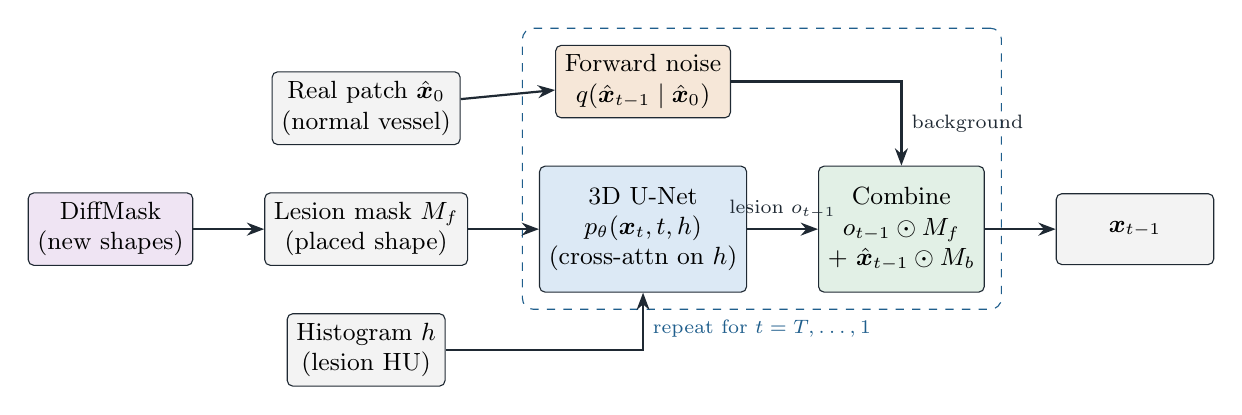
\begin{tikzpicture}[node distance=6mm and 9mm]
\node[blkE] (mf) {Lesion mask $M_f$\\(placed shape)};
\node[blkE, above=of mf] (x0) {Real patch $\hat\x_0$\\(normal vessel)};
\node[blkE, below=of mf] (h) {Histogram $h$\\(lesion HU)};
\node[blkD, left=9mm of mf] (dm) {DiffMask\\(new shapes)};
\node[blkA, right=of mf, minimum height=16mm] (unet) {3D U-Net\\$p_\theta(\x_t,t,h)$\\(cross-attn on $h$)};
\node[blkB, above=of unet] (fwd) {Forward noise\\$q(\hat\x_{t-1}\mid\hat\x_0)$};
\node[blkC, right=of unet, minimum height=16mm] (mix) {Combine\\$o_{t-1}\had M_f$\\$+\ \hat\x_{t-1}\had M_b$};
\node[blkE, right=of mix] (out) {$\x_{t-1}$};
\draw[arr] (dm)--(mf);
\draw[arr] (x0)--(fwd);
\draw[arr] (fwd) -| node[lbl,pos=0.75,right]{background} (mix);
\draw[arr] (mf)--(unet);
\draw[arr] (h) -| (unet);
\draw[arr] (unet)--node[lbl,above]{lesion $o_{t-1}$} (mix);
\draw[arr] (mix)--(out);
\begin{scope}[on background layer]
\node[grp, fit=(unet)(mix)(fwd), label={[lbl,text=acc]below:repeat for $t=T,\dots,1$}] {};
\end{scope}
\end{tikzpicture}
\end{adjustbox}
\caption{LeFusion (redrawn). The U-Net only generates the lesion; the background is a noised copy of the real patch at each step.}
\end{figure}


\subsection*{A.4 Maths and loss}
\textbf{Generation step (paper Eq.~1).} Same as Eq.~\eqref{eq:lef-inp}, with lesion mask $M_f$ and background mask $M_b=1-M_f$:
\begin{equation}
\x_{t-1} = o_{t-1}\had M_f + \hat\x_{t-1}\had M_b,\qquad o_{t-1}\sim p_\theta(\x_t,t),\qquad \hat\x_{t-1}\sim q(\hat\x_0,t).
\end{equation}

\textbf{Lesion-focused loss (paper Eq.~2).} The loss counts only voxels inside the lesion:
\begin{equation}
\Loss_{\text{LeF}} = \E_{\hat\x_0,\eps,t}\Big[\,M_f\had\norm{\eps-\eps_\theta(\hat\x_t,t)}_2\Big].
\end{equation}
\emph{Why:} most voxels in a patch are background, and the background is copied anyway. So all learning goes to the lesion.

\textbf{Histogram control (paper Eq.~3).} A histogram $h$ of lesion brightness is given through cross-attention:
\begin{equation}
o_{t-1}\sim p_\theta(\x_t,h,t).
\end{equation}
Change $h$ $\rightarrow$ the lesion becomes brighter or darker.

\textbf{Several lesion types (paper Eq.~4).} One mask channel per type $i=1..n$:
\begin{equation}
\Loss = \E\sum_{i=1}^{n}\Big[M_f^{(i)}\had\norm{\eps-\eps_\theta(\hat\x_t,t)}_2^{(i)}\Big].
\end{equation}

\textbf{DiffMask.} A separate diffusion model that makes mask shapes. It gets a ``control sphere'' (where and how big) and returns a realistic shape inside it.

\subsection*{A.5 Input and output}
\begin{center}
\small
\begin{tabularx}{\linewidth}{lX}
\toprule
\textbf{Training input} & real lesion patch, its mask $M_f$, histogram $h$ \\
\textbf{Generation input} & normal patch, a mask $M_f$, a histogram $h$ \\
\textbf{Output} & patch with a new lesion inside $M_f$; background unchanged \\
\textbf{Loss} & $\Loss_{\text{LeF}}$ (noise error inside the lesion only) \\
\bottomrule
\end{tabularx}
\end{center}

\subsection*{A.6 Results in the paper}
Lung nodules (LIDC), Dice: nnU-Net 78.26 $\rightarrow$ 83.44; SwinUNETR 78.38 $\rightarrow$ 83.13 when LeFusion data is added. Training: 3$\times$A100 for about 1 day. About 30\,s per sample.

\section{Part B -- Our dataset}

\subsection*{B.1 What data this method needs}
\begin{itemize}
  \item $\approx$1{,}300 aneurysm patches ($64^3$) with masks -- from Common Steps 1--4.
  \item $\approx$5{,}000 normal vessel patches -- the places where new aneurysms go.
  \item The shape library (Step 5) -- to train DiffMask. Masks without scans can be used here.
\end{itemize}

\subsection*{B.2 How we train it}
\begin{center}
\small
\begin{tabularx}{\linewidth}{lX}
\toprule
\textbf{Part} & \textbf{Choice} \\
\midrule
LeFusion U-Net & \textbf{train from scratch}, all layers. (Option: start from the released lung model and fine-tune all layers. Do not freeze anything: the anatomy is different.) \\
DiffMask & \textbf{train from scratch} on our mask shapes \\
LoRA & \textbf{not needed} -- the model is mid-size, not a huge pretrained model \\
\bottomrule
\end{tabularx}
\end{center}

\subsection*{B.3 Step-by-step pipeline}
\begin{enumerate}
  \item Run Common Steps 1--5.
  \item For each aneurysm patch, compute $h$: a 16-bin histogram of HU inside the mask.
  \item Change the paper's patch size $64\times64\times32$ to $64^3$ (our voxels are about the same size in all directions).
  \item \textbf{Train LeFusion}: $T=1000$ steps (cosine schedule), batch 4--8, AdamW, learning rate $10^{-4}$, about 100k iterations, EMA 0.999, random flips and $90^\circ$ rotations.
  \item \textbf{Train DiffMask} on the shape library, with a control sphere of the wanted size.
  \item \textbf{Generate}: pick a normal vessel patch $\rightarrow$ choose a place (Step 6) $\rightarrow$ get a shape (DiffMask or library) $\rightarrow$ pick $h$ from real histograms $\rightarrow$ run LeFusion.
  \item Put the patch back into the full scan and save (Step 7).
\end{enumerate}

\subsection*{B.4 Compute}
One GPU with 24--40\,GB. Training about 1--3 days (estimate). Generation about 30\,s per aneurysm (paper).

\subsection*{B.5 How to check it worked}
\begin{itemize}
  \item Look at 30--50 results with the visualisation notebook. The aneurysm should grow from the vessel, with no seam.
  \item Compare HU inside synthetic vs.\ real aneurysms (mean, spread).
  \item Copy check: no synthetic aneurysm should be almost identical to a training one.
  \item Then the full test in Chapter~\ref{ch:eval}.
\end{itemize}

\subsection*{B.6 Risks}
\begin{caution}
The mask edge must touch a bright vessel, or the result is a ``floating blob''. Placement (Step 6) matters as much as the model. In Case A (117 aneurysms) the model may copy training examples; use Case A only to test the code.
\end{caution}

\subsection*{B.7 Rank for our dataset}
\begin{verdict}{Rank 1 of 8 -- best fit}
\begin{tabular}{ll}
Small-lesion detail & \stars{5} (full resolution)\\
Fits our data size & \stars{4}\\
Compute (5 = cheap) & \stars{4}\\
Code available & \stars{4}\\
Mask is exact & \stars{5}\\
Effort (5 = easy) & \stars{3}\\
\end{tabular}

\smallskip
Built for exactly this job: small lesions inside real CT, at full resolution, with brightness control and new shapes.
\end{verdict}

% =================== METHOD 2: DiffTumor ===================
\chapter{Method 2 -- DiffTumor}\label{ch:difftumor}

\section{Part A -- The paper}

\subsection*{A.1 Idea}
\begin{idea}
First train a 3D autoencoder that compresses CT. Then train a diffusion model on the compressed version that fills a masked area with a lesion, using the healthy area around it as a guide. Decode and paste the lesion into a healthy scan.
\end{idea}
\textbf{Paper.} Q.~Chen, X.~Chen, H.~Song, \emph{et al.}, ``Towards Generalizable Tumor Synthesis'', CVPR 2024~\cite{chen2024difftumor}. Code and trained models: \url{https://github.com/MrGiovanni/DiffTumor}. Key message: small, early lesions look alike in different organs, so the model generalises.

\subsection*{A.2 Basics you need: autoencoders and latent diffusion}
\textbf{Autoencoder.} An encoder $\enc$ makes a small code $\z=\enc(\x)$, $f$ times smaller per axis. A decoder makes the image back: $\hat\x=\dec(\z)$. Training makes $\hat\x$ close to $\x$.

\textbf{VQ (vector quantisation).} Each code vector is replaced by the nearest entry $\bm c_z$ in a learned ``codebook''~\cite{esser2021vqgan}. Loss for this (sg = stop gradient):
\begin{equation}
\Loss_{\text{VQ}} = \norm{\sg[\enc(\x)]-\bm c_z}_2^2 + \gamma\,\norm{\sg[\bm c_z]-\enc(\x)}_2^2 .
\end{equation}

\textbf{Latent diffusion.} Run the diffusion model (Eq.~\eqref{eq:lef-q}--\eqref{eq:lef-rev} in Chapter~\ref{ch:lefusion}) on $\z$ instead of $\x$~\cite{rombach2022ldm}. It is faster and uses less memory.

\textbf{Catch for us.} With $f=4$, a 5\,mm aneurysm (11 voxels) becomes about 3 code voxels. Fine detail can be lost.

\subsection*{A.3 Architecture}
\begin{figure}[H]
\centering
\begin{adjustbox}{max width=\linewidth}
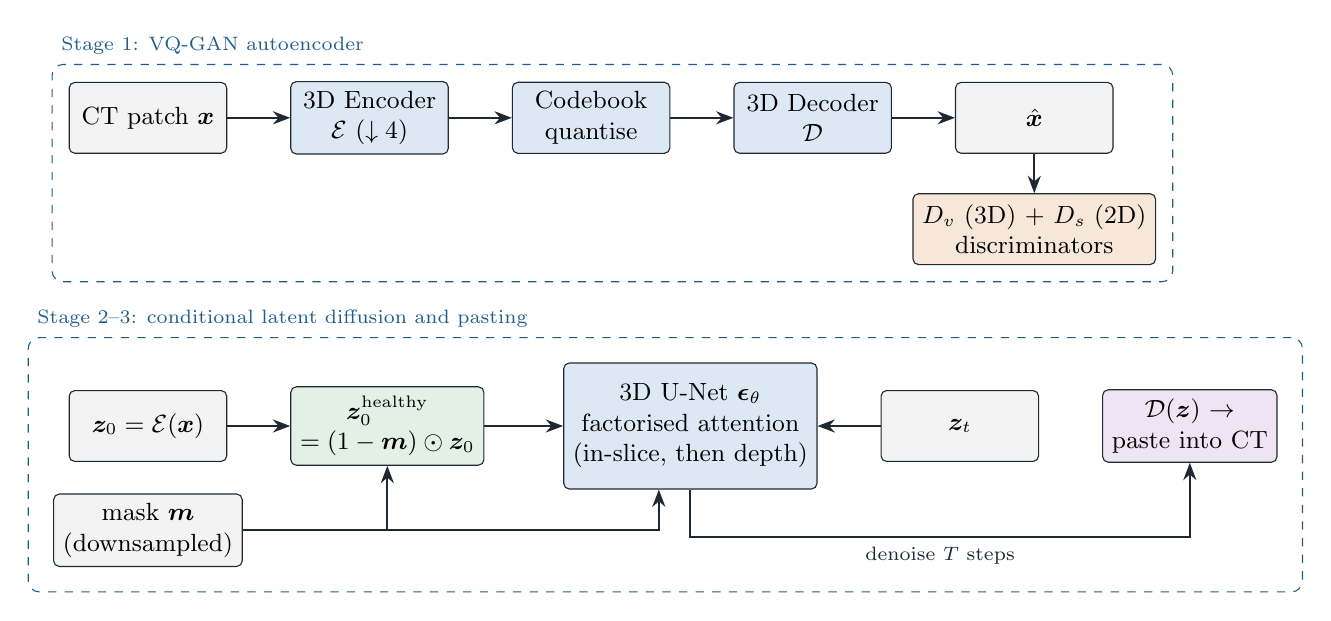
\begin{tikzpicture}[node distance=6mm and 8mm]
% stage 1
\node[blkE] (x) {CT patch $\x$};
\node[blkA, right=of x] (E) {3D Encoder\\$\enc$ ($\downarrow 4$)};
\node[blkA, right=of E] (Q) {Codebook\\quantise};
\node[blkA, right=of Q] (Dd) {3D Decoder\\$\dec$};
\node[blkE, right=of Dd] (xh) {$\hat\x$};
\node[blkB, below=5mm of xh, minimum width=24mm] (disc) {$D_v$ (3D) + $D_s$ (2D)\\discriminators};
\draw[arr] (x)--(E); \draw[arr] (E)--(Q); \draw[arr] (Q)--(Dd); \draw[arr] (Dd)--(xh); \draw[arr] (xh)--(disc);
\node[grp, fit=(x)(E)(Q)(Dd)(xh)(disc), label={[lbl,text=acc,anchor=south west]north west:Stage 1: VQ-GAN autoencoder}] (s1) {};
% stage 2
\node[blkE, below=30mm of x] (z0) {$\z_0=\enc(\x)$};
\node[blkE, below=4mm of z0] (mm) {mask $\m$\\(downsampled)};
\node[blkC, right=of z0] (zh) {$\z_0^{\text{healthy}}$\\$=(1-\m)\had\z_0$};
\node[blkA, right=10mm of zh, minimum height=16mm] (unet) {3D U-Net $\eps_\theta$\\factorised attention\\(in-slice, then depth)};
\node[blkE, right=of unet] (zt) {$\z_t$};
\node[blkD, right=of zt] (dec2) {$\dec(\z)$ $\rightarrow$\\paste into CT};
\draw[arr] (z0)--(zh); \draw[arr] (mm) -| (zh); \draw[arr] (zh)--(unet); \draw[arr] (mm.east) -| ([xshift=-4mm]unet.south);
\draw[arr] (zt)--(unet); \draw[arr] (unet.south) |- ++(0,-6mm) -| node[lbl,pos=0.25,below]{denoise $T$ steps} (dec2.south);
\node[grp, fit=(z0)(mm)(zh)(unet)(zt)(dec2), inner sep=9pt, label={[lbl,text=acc,anchor=south west]north west:Stage 2--3: conditional latent diffusion and pasting}] {};
\end{tikzpicture}
\end{adjustbox}
\caption{DiffTumor (redrawn). Stage 1 learns a compact CT code. Stage 2 fills the masked latent with a lesion, conditioned on the healthy latent and the mask.}
\end{figure}


\subsection*{A.4 Maths and loss}
\textbf{Stage 1 -- autoencoder (paper Eq.~2).} A 3D VQ-GAN, compression 4 per axis, codebook of 16{,}384 entries:
\begin{equation}
\min_{\enc,\dec,C}\Big(\Loss_{\text{recon}}+\Loss_{\text{VQ}}+\Loss_{\text{match}}+\Loss_{\text{perc}}\Big) + \min_{\enc,\dec,C}\max_{D_s,D_v}\Loss_{\text{disc}},
\end{equation}
\begin{align}
\Loss_{\text{recon}} &= \norm{\x-\hat\x}_1, &
\Loss_{\text{disc}} &= \log D(\x) + \log\big(1-D(\hat\x)\big),\\
\Loss_{\text{match}} &= \textstyle\sum_i\norm{D^{(i)}(\hat\x)-D^{(i)}(\x)}_1, &
\Loss_{\text{perc}} &= \text{perceptual loss on 2D slices}.
\end{align}
$D_v$ judges 3D volumes, $D_s$ judges 2D slices.

\textbf{Stage 2 -- diffusion (paper Eq.~6).} The model sees the noisy code $\z_t$, the healthy code $\z_0^{\text{healthy}}=(1-\m)\had\z_0$, and the mask $\m$:
\begin{equation}
\Loss_{\text{diff}} = \E_{\z_0,\eps,t}\Big[\norm{\eps-\eps_\theta(\z_t,\ \z_0^{\text{healthy}},\ \m,\ t)}_2^2\Big].
\end{equation}
The U-Net uses split attention: first inside each slice, then across slices. Generation uses very few steps (default $T=4$, $\approx$0.2\,s per lesion).

\textbf{Stage 3.} Decode and paste into a healthy scan. Paper masks are ellipsoids.

\subsection*{A.5 Input and output}
\begin{center}
\small
\begin{tabularx}{\linewidth}{lX}
\toprule
\textbf{Autoencoder} & CT patch in $\rightarrow$ same patch out \\
\textbf{Diffusion input} & noisy code, healthy code, mask, step $t$ \\
\textbf{Output} & CT patch with a new lesion; mask = $\m$ \\
\textbf{Losses} & AE: $L_1$ + VQ + perceptual + adversarial + feature match. Diffusion: $\Loss_{\text{diff}}$ \\
\bottomrule
\end{tabularx}
\end{center}

\subsection*{A.6 Results in the paper}
Dice (\%), real $\rightarrow$ real + DiffTumor, U-Net: liver 62.3 $\rightarrow$ 70.9; pancreas 56.0 $\rightarrow$ 64.8; kidney 75.1 $\rightarrow$ 84.2. Autoencoder trained on 9{,}262 CT scans (1\,mm, $96^3$ crops, HU $[-175,250]$).

\section{Part B -- Our dataset}

\subsection*{B.1 What data this method needs}
\begin{itemize}
  \item Many patches (aneurysm + normal vessel, $\approx$6{,}000+) for the autoencoder.
  \item $\approx$1{,}300 aneurysm patches with masks for the diffusion model.
  \item Shape library (Step 5) for masks at generation time (better than ellipsoids).
\end{itemize}

\subsection*{B.2 How we train it}
\begin{center}
\small
\begin{tabularx}{\linewidth}{lXX}
\toprule
\textbf{Part} & \textbf{Quick option} & \textbf{Better option (recommended)} \\
\midrule
Autoencoder & start from released CT model; \textbf{fine-tune all layers} with our HU range & \textbf{train from scratch} with compression 2 (not 4), so small aneurysms keep detail \\
Diffusion U-Net & \textbf{train from scratch} & \textbf{train from scratch} \\
LoRA & not useful (models are mid-size, data looks very different) & not useful \\
\bottomrule
\end{tabularx}
\end{center}

\subsection*{B.3 Step-by-step pipeline}
\begin{enumerate}
  \item Run Common Steps 1--5.
  \item \textbf{Train the autoencoder} on all patches (HU $[-100,900]\rightarrow[-1,1]$).
  \item \textbf{Test the autoencoder on aneurysms}: encode and decode 50 aneurysm patches; the aneurysm (threshold at vessel HU) should keep Dice $\ge0.85$. If not, the autoencoder is too lossy -- use compression 2.
  \item \textbf{Encode} all aneurysm patches. Shrink masks with max-pooling so small masks do not disappear.
  \item \textbf{Train the diffusion model} with $\Loss_{\text{diff}}$, $T=1000$. Generate with 50 DDIM steps (safer than 4 for a new kind of data).
  \item \textbf{Generate}: normal vessel patch + placed mask (Step 6, shape from library) $\rightarrow$ new aneurysm.
  \item Put back and save (Step 7).
\end{enumerate}

\subsection*{B.4 Compute}
Paper: autoencoder 4$\times$A100 for about a week; diffusion 1$\times$A100 for about a day. Ours (estimate): autoencoder 3--7 days and diffusion about 1 day on one 40\,GB GPU. Generation is under a second.

\subsection*{B.5 How to check it worked}
\begin{itemize}
  \item Autoencoder test in step 3 (most important).
  \item Background HU before vs.\ after: decoding may shift it slightly.
  \item Visual check and copy check, then Chapter~\ref{ch:eval}.
\end{itemize}

\subsection*{B.6 Risks}
\begin{caution}
Compression is the main risk: with compression 4, a 3\,mm aneurysm is 1--2 code voxels. Also, decoding can change the background a little, so always paste with the soft mask.
\end{caution}

\subsection*{B.7 Rank for our dataset}
\begin{verdict}{Rank 2 of 8}
\begin{tabular}{ll}
Small-lesion detail & \stars{3} (better with compression 2)\\
Fits our data size & \stars{4}\\
Compute (5 = cheap) & \stars{3}\\
Code available & \stars{5}\\
Mask is exact & \stars{4}\\
Effort (5 = easy) & \stars{3}\\
\end{tabular}

\smallskip
Most mature code. Second only because compression can blur tiny aneurysms. First backup if LeFusion has problems.
\end{verdict}

% =================== METHOD 3: 3D cGAN ===================
\chapter{Method 3 -- 3D conditional GAN (Jin et al.)}\label{ch:cgan}

\section{Part A -- The paper}

\subsection*{A.1 Idea}
\begin{idea}
Erase the centre of a 3D CT box. A generator fills it back in. A discriminator judges if the result looks real. If the erased part held a lesion, the generator learns to draw lesions that blend in.
\end{idea}
\textbf{Paper.} D.~Jin, Z.~Xu, Y.~Tang, \emph{et al.}, ``CT-Realistic Lung Nodule Simulation from 3D Conditional Generative Adversarial Networks for Robust Lung Segmentation'', MICCAI 2018~\cite{jin2018cgan}. Code: not released.

\subsection*{A.2 Basics you need: GANs}
A GAN has two networks~\cite{goodfellow2014gan}. The \textbf{generator} $G$ makes images. The \textbf{discriminator} $D$ says ``real'' or ``fake''. They compete: $G$ tries to fool $D$. In a \emph{conditional} GAN~\cite{isola2017pix2pix}, both also see an input $\bm x$ (here: the box with a hole):
\begin{equation}\label{eq:cgan-basic}
\Loss_{\text{cGAN}}(G,D)=\E_{\bm x,\bm y}\big[\log D(\bm x,\bm y)\big]+\E_{\bm x}\big[\log\big(1-D(\bm x,G(\bm x))\big)\big].
\end{equation}
GANs are very fast at generation (one pass), but harder to train than diffusion, and can produce too little variety (``mode collapse'').

\subsection*{A.3 Architecture}
\begin{figure}[H]
\centering
\begin{adjustbox}{max width=\linewidth}
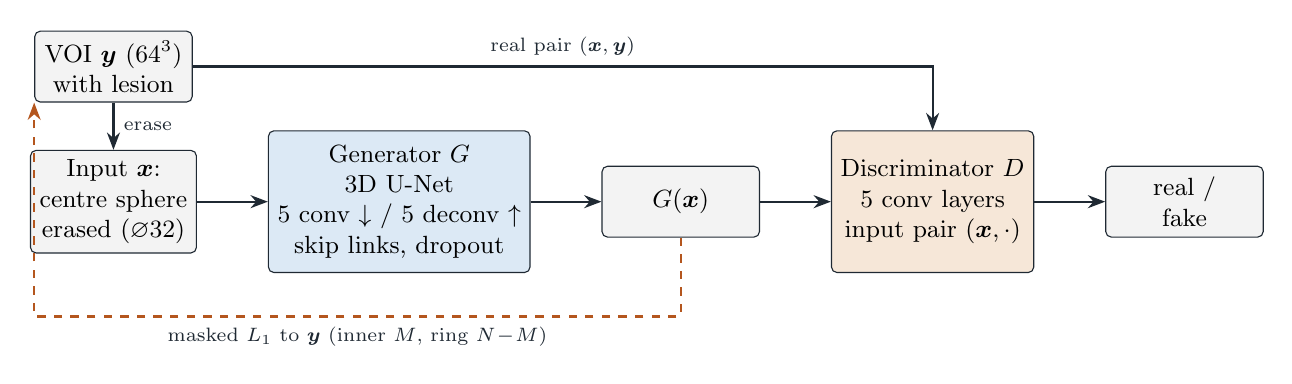
\begin{tikzpicture}[node distance=6mm and 9mm]
\node[blkE] (y) {VOI $\bm y$ ($64^3$)\\with lesion};
\node[blkE, below=of y] (xin) {Input $\bm x$:\\centre sphere\\erased ($\varnothing32$)};
\node[blkA, right=of xin, minimum height=18mm] (G) {Generator $G$\\3D U-Net\\5 conv $\downarrow$ / 5 deconv $\uparrow$\\skip links, dropout};
\node[blkE, right=of G] (gx) {$G(\bm x)$};
\node[blkB, right=of gx, minimum height=18mm] (D) {Discriminator $D$\\5 conv layers\\input pair $(\bm x,\cdot)$};
\node[blkE, right=of D] (rf) {real /\\fake};
\draw[arr] (y)--(xin) node[midway,lbl,right]{erase};
\draw[arr] (xin)--(G); \draw[arr] (G)--(gx); \draw[arr] (gx)--(D); \draw[arr] (D)--(rf);
\draw[arr] (y) -| node[lbl,pos=0.25,above]{real pair $(\bm x,\bm y)$} (D);
\draw[darr] (gx.south) |- ++(0,-10mm) -| node[lbl,pos=0.25,below]{masked $L_1$ to $\bm y$ (inner $M$, ring $N\!-\!M$)} (y.south west);
\end{tikzpicture}
\end{adjustbox}
\caption{3D cGAN inpainting (redrawn from Jin et al.). The generator fills the erased sphere; losses push the fill to match the real lesion and to look real to $D$.}
\end{figure}


\textbf{Details.} Boxes of $64\times64\times64$. The hole is a sphere of 32 voxels across. $G$: 3D U-Net (5 layers down, 5 up, skip links); dropout is the only randomness. $D$: 5 convolution layers.

\subsection*{A.4 Maths and loss}
\textbf{Adversarial loss}: Eq.~\eqref{eq:cgan-basic}.

\textbf{Two-zone $L_1$ loss.} $M$ = the hole. $N$ = the hole grown by 3--6 voxels, so $N-M$ is a ring around it:
\begin{equation}
\Loss_{L_1}(G) = \E\Big[M\had\norm{\bm y-G(\bm x)}_1\Big] + \alpha\,\E\Big[(N-M)\had\norm{\bm y-G(\bm x)}_1\Big],\qquad \alpha=5.
\end{equation}
The ring gets 5$\times$ more weight, so the edge blends smoothly.

\textbf{Total:}
\begin{equation}
G^\star = \arg\min_G\max_D\ \Loss_{\text{cGAN}}(G,D) + \lambda\,\Loss_{L_1}(G),\qquad \lambda=100.
\end{equation}
Adam, learning rate $10^{-4}$, $\beta_1=0.5$; 12 epochs; $\approx$4{,}300 training boxes.

\subsection*{A.5 Input and output}
\begin{center}
\small
\begin{tabularx}{\linewidth}{lX}
\toprule
\textbf{Input} & $64^3$ box with the centre sphere erased \\
\textbf{Output} & the full $64^3$ box, hole filled \\
\textbf{Loss} & cGAN loss + $100\times$ two-zone $L_1$ \\
\bottomrule
\end{tabularx}
\end{center}

\subsection*{A.6 Results in the paper}
Lung segmentation Dice on scans with nodules at the lung edge: 0.964 $\rightarrow$ 0.989 after adding simulated nodules.

\section{Part B -- Our dataset}

\subsection*{B.1 What data this method needs}
$\approx$1{,}300 aneurysm patches ($64^3$) with masks; normal vessel patches for generation; shape library.

\subsection*{B.2 How we train it}
\textbf{Train from scratch, all layers.} No pretrained model exists and the model is small. LoRA is not relevant.

\textbf{Two changes we make to the paper:}
\begin{enumerate}
  \item \textbf{Hole shaped like the aneurysm}: erase the mask grown by 2 voxels, not a fixed sphere.
  \item \textbf{Give the mask as an extra input channel}, and add a loss that makes the bright part match the mask:
  \begin{equation}
  \Loss_{\text{mask}} = \operatorname{BCE}\Big(\sigma\big(k\,(G(\bm x)-\tau)\big),\ \m\Big)\ \text{ inside } N .
  \end{equation}
  $\tau$ = vessel brightness level, $k$ = sharpness. This makes the drawn aneurysm follow the mask, so the mask is correct.
\end{enumerate}

\subsection*{B.3 Step-by-step pipeline}
\begin{enumerate}
  \item Run Common Steps 1--5.
  \item Build training pairs: target $\bm y$ = aneurysm patch; input $\bm x$ = same patch with the grown mask erased + mask channel.
  \item \textbf{Train} with $\Loss_{\text{cGAN}} + 100\,\Loss_{L_1} + \lambda_m\Loss_{\text{mask}}$ ($\lambda_m$ = 1--10). Use spectral normalisation in $D$ for stable training. Batch 8--16.
  \item \textbf{Generate}: normal vessel patch + placed mask (Step 6) $\rightarrow$ erase $\rightarrow$ $G$.
  \item Put back and save (Step 7).
\end{enumerate}

\subsection*{B.4 Compute}
One 16--24\,GB GPU. Training under 1 day (estimate). Generation takes milliseconds.

\subsection*{B.5 How to check it worked}
\begin{itemize}
  \item Variety: generate 10 aneurysms for the \emph{same} mask. If all look the same, variety is low.
  \item Check that bright voxels match the mask (Dice of thresholded output vs.\ mask).
  \item Visual check, then Chapter~\ref{ch:eval}.
\end{itemize}

\subsection*{B.6 Risks}
\begin{caution}
GAN training can be unstable, and dropout is the only randomness, so results can look alike. Variety then comes mostly from the shape library and placement.
\end{caution}

\subsection*{B.7 Rank for our dataset}
\begin{verdict}{Rank 3 of 8 -- fast baseline}
\begin{tabular}{ll}
Small-lesion detail & \stars{4}\\
Fits our data size & \stars{4}\\
Compute (5 = cheap) & \stars{5}\\
Code available & \stars{2} (simple to write)\\
Mask is exact & \stars{3} (needs our changes)\\
Effort (5 = easy) & \stars{4}\\
\end{tabular}

\smallskip
Cheap and quick. A good first generative baseline to compare the diffusion methods against.
\end{verdict}

% =================== METHOD 4: RePaint ===================
\chapter{Method 4 -- RePaint}\label{ch:repaint}

\section{Part A -- The paper}

\subsection*{A.1 Idea}
\begin{idea}
Train a normal diffusion model (no mask input). To fill a hole: at each step keep the real part, let the model draw only inside the hole, and go back and forth a few times so the two parts blend.
\end{idea}
\textbf{Paper.} A.~Lugmayr, M.~Danelljan, A.~Romero, \emph{et al.}, ``RePaint: Inpainting using Denoising Diffusion Probabilistic Models'', CVPR 2022~\cite{lugmayr2022repaint}. Code (2D photos): \url{https://github.com/andreas128/RePaint}.

\subsection*{A.2 Basics you need}
A standard diffusion model, trained with the plain loss of Eq.~\eqref{eq:lef-ddpm} (Chapter~\ref{ch:lefusion}), \emph{without} any condition. RePaint does not change training at all; it only changes how we generate.

\subsection*{A.3 Architecture}
\begin{figure}[H]
\centering
\begin{adjustbox}{max width=\linewidth}
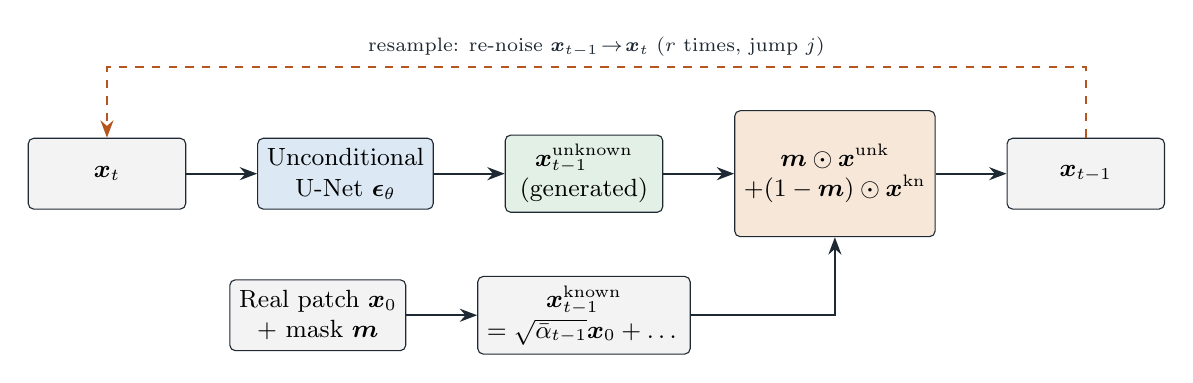
\begin{tikzpicture}[node distance=6mm and 9mm]
\node[blkE] (xt) {$\x_t$};
\node[blkA, right=of xt] (unet) {Unconditional\\U-Net $\eps_\theta$};
\node[blkC, right=of unet] (unk) {$\x^{\text{unknown}}_{t-1}$\\(generated)};
\node[blkE, below=8mm of unk] (kn) {$\x^{\text{known}}_{t-1}$\\$=\sqrt{\abar_{t-1}}\x_0+\dots$};
\node[blkE, left=of kn] (x0) {Real patch $\x_0$\\+ mask $\m$};
\node[blkB, right=of unk, minimum height=16mm] (mix) {$\m\had\x^{\text{unk}}$\\$+(1-\m)\had\x^{\text{kn}}$};
\node[blkE, right=of mix] (xt1) {$\x_{t-1}$};
\draw[arr] (xt)--(unet); \draw[arr] (unet)--(unk); \draw[arr] (unk)--(mix);
\draw[arr] (x0)--(kn); \draw[arr] (kn) -| (mix); \draw[arr] (mix)--(xt1);
\draw[darr] (xt1.north) |- ++(0,9mm) -| node[lbl,pos=0.25,above]{resample: re-noise $\x_{t-1}\!\rightarrow\!\x_t$ ($r$ times, jump $j$)} (xt.north);
\end{tikzpicture}
\end{adjustbox}
\caption{RePaint (redrawn). Known region from the real image, unknown region from the model; re-noising lets both parts agree.}
\end{figure}


\subsection*{A.4 Maths}
With $\m=1$ in the hole:
\begin{align}
\x_{t-1}^{\text{known}} &\sim \N\big(\sqrt{\abar_{t-1}}\,\x_0,\ (1-\abar_{t-1})\I\big) && \text{(real image, noised)}\\
\x_{t-1}^{\text{unknown}} &\sim \N\big(\bm\mu_\theta(\x_t,t),\ \Sigma_\theta(\x_t,t)\big) && \text{(model's guess)}\\
\x_{t-1} &= \m\had\x_{t-1}^{\text{unknown}} + (1-\m)\had\x_{t-1}^{\text{known}} .
\end{align}
\textbf{Going back (resampling).} The two parts may not match at the edge. So add one step of noise back,
\begin{equation}
\x_t \sim \N\big(\sqrt{1-\beta_t}\,\x_{t-1},\ \beta_t\I\big),
\end{equation}
and denoise again. Repeat $r$ times, in jumps of $j$ steps. Paper: $T=250$, $j=10$, $r=10$. This makes generation about $10\times$ slower.

\subsection*{A.5 Input and output}
\begin{center}
\small
\begin{tabularx}{\linewidth}{lX}
\toprule
\textbf{Training input} & images only (no masks) \\
\textbf{Training loss} & plain diffusion loss \\
\textbf{Generation input} & real image + hole mask \\
\textbf{Output} & image with new content in the hole \\
\bottomrule
\end{tabularx}
\end{center}

\subsection*{A.6 Results in the paper}
Strong results for 2D photo inpainting with many hole shapes. Not tested on medical lesions in the paper.

\section{Part B -- Our dataset}

\subsection*{B.1 What data this method needs}
$\approx$1{,}300 aneurysm patches ($64^3$) for training (masks not needed for training); normal vessel patches and the shape library for generation.

\subsection*{B.2 How we train it}
\textbf{Train a 3D diffusion model from scratch, all layers.} No 3D head-CTA diffusion model exists to reuse. LoRA is not relevant. Filling the hole needs no extra training.

\subsection*{B.3 Step-by-step pipeline}
\begin{enumerate}
  \item Run Common Steps 1--5.
  \item \textbf{Train} a 3D diffusion model on aneurysm-centred patches only ($T=1000$, cosine). Training only on aneurysm patches teaches the model to ``expect'' a bright blob near the centre.
  \item \textbf{Generate} with RePaint ($T=250$, $j=10$, $r=10$) on a normal vessel patch, hole = placed mask grown by 1--2 voxels.
  \item (Optional) push the hole to be bright with a small guidance step:
  \begin{equation}
  \x^{\text{unk}}_{t-1} \leftarrow \x^{\text{unk}}_{t-1} - \eta\,\nabla_{\x}\big(\text{mean of }\hat\x_0\text{ inside }\m - \mu_a\big)^2 .
  \end{equation}
  \item \textbf{Fix the mask}: the model may not fill the whole hole with aneurysm, so keep only bright voxels:
  \begin{equation}
  \m^{\text{final}} = \m \wedge (\hat\x > \tau_v).
  \end{equation}
  Throw away results where $\m^{\text{final}}$ is under 70\% of $\m$.
  \item Put back and save (Step 7).
\end{enumerate}

\subsection*{B.4 Compute}
One 24\,GB GPU; training 1--3 days (estimate). Generation about 10$\times$ slower than normal diffusion.

\subsection*{B.5 How to check it worked}
Count how many results are thrown away in step 5 (high = poor control). Then visual check and Chapter~\ref{ch:eval}.

\subsection*{B.6 Risks}
\begin{caution}
The model is never told ``draw an aneurysm here''. It may fill the hole with brain or plain vessel. This is the weakest control of the four mask-filling methods.
\end{caution}

\subsection*{B.7 Rank for our dataset}
\begin{verdict}{Rank 4 of 8}
\begin{tabular}{ll}
Small-lesion detail & \stars{4}\\
Fits our data size & \stars{3}\\
Compute (5 = cheap) & \stars{3} (slow generation)\\
Code available & \stars{3} (2D only; port to 3D)\\
Mask is exact & \stars{2}\\
Effort (5 = easy) & \stars{4}\\
\end{tabular}

\smallskip
Simple and well known. Useful as a diffusion baseline to show how much LeFusion's lesion-focused training helps.
\end{verdict}

% =================== METHOD 5: MAISI ===================
\chapter{Method 5 -- MAISI / MAISI-v2 with ControlNet and LoRA}\label{ch:maisi}

\section{Part A -- The paper}

\subsection*{A.1 Idea}
\begin{idea}
Use NVIDIA's large, already-trained 3D CT generator. Keep it frozen. Train a small add-on (ControlNet) so a label map (vessels + aneurysm) controls what it draws. Optionally adapt the big model to head CTA with LoRA.
\end{idea}
\textbf{Papers.} P.~Guo, C.~Zhao, D.~Yang, \emph{et al.}, ``MAISI: Medical AI for Synthetic Imaging'', WACV 2025~\cite{guo2025maisi}. C.~Zhao, P.~Guo, D.~Yang, \emph{et al.}, ``MAISI-v2'', arXiv 2025~\cite{zhao2025maisiv2}. Code (Apache-2.0): \url{https://github.com/NVIDIA-Medtech/NV-Generate-CTMR}. Model weights: NVIDIA Open Model licence.

\subsection*{A.2 Basics you need}
\textbf{Latent diffusion}: see Chapter~\ref{ch:difftumor}, A.2.

\textbf{Rectified flow} (used by MAISI-v2)~\cite{liu2023rf}. Instead of guessing noise, learn a ``speed'' that moves noise $\x_0$ to an image $\x_1$ along a straight line:
\begin{equation}\label{eq:maisi-rf}
\x_t=(1-t)\,\x_0+t\,\x_1,\qquad
\Loss_{\text{flow}}=\E\Big[\norm{\bm v_\theta(\x_t,t,\bm c)-(\x_1-\x_0)}_2^2\Big].
\end{equation}
Straight lines mean good images in about 30 steps instead of 1000.

\textbf{ControlNet}~\cite{zhang2023controlnet}. Copy the encoder of the frozen U-Net into a trainable copy. Feed it the label map $\bm c$. Join it to the frozen model with ``zero convolutions'' $\mathcal Z$ that start at zero:
\begin{equation}
\bm y_c = \mathcal F(\x;\Theta) + \mathcal Z\Big(\mathcal F\big(\x+\mathcal Z(\bm c;\Theta_{z1});\Theta_c\big);\Theta_{z2}\Big).
\end{equation}
$\Theta$ is frozen; only $\Theta_c,\Theta_{z1},\Theta_{z2}$ learn. At the start the add-on outputs zero, so nothing breaks.

\textbf{LoRA}~\cite{hu2022lora}. Fine-tune a big frozen weight $W_0$ cheaply by adding a small low-rank update:
\begin{equation}
W = W_0 + \frac{\alpha}{r}\,BA,\qquad B\in\R^{d\times r},\ A\in\R^{r\times k},\ r\ll d,k .
\end{equation}
Only $A$ and $B$ are trained (often under 1\% of the weights). $B$ starts at zero.

\subsection*{A.3 Architecture}
\begin{figure}[H]
\centering
\begin{adjustbox}{max width=\linewidth}
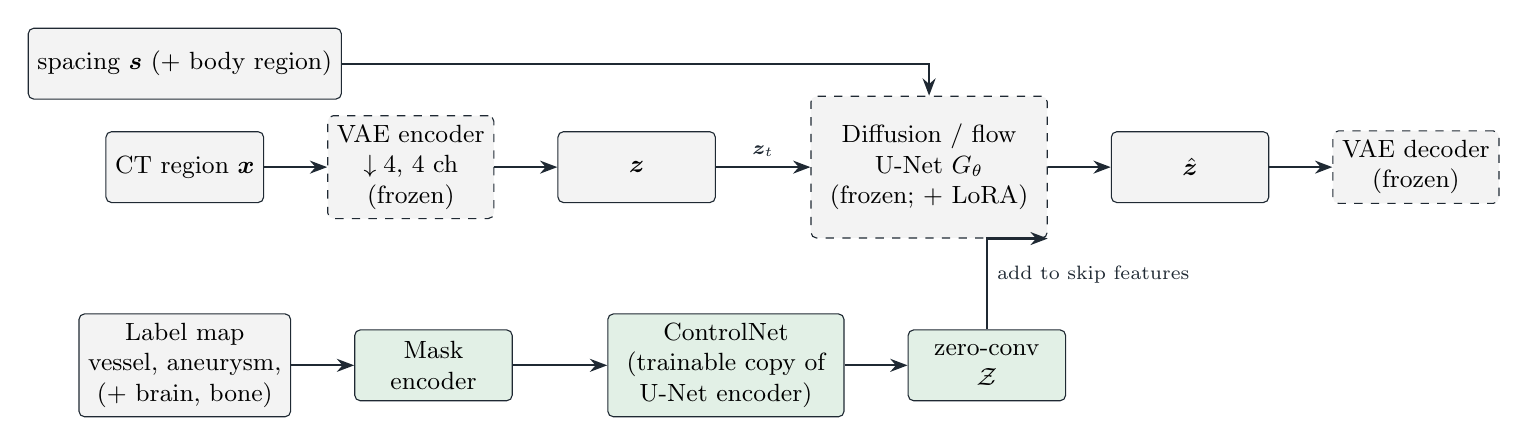
\begin{tikzpicture}[node distance=6mm and 8mm]
\node[blkE] (x) {CT region $\x$};
\node[frz, right=of x] (E) {VAE encoder\\$\downarrow4$, 4 ch\\(frozen)};
\node[blkE, right=of E] (z) {$\z$};
\node[frz, right=12mm of z, minimum height=18mm, minimum width=30mm] (U) {Diffusion / flow\\U-Net $G_\theta$\\(frozen; + LoRA)};
\node[blkE, right=of U] (zh) {$\hat\z$};
\node[frz, right=of zh] (Dd) {VAE decoder\\(frozen)};
\node[blkE, below=14mm of x] (lab) {Label map\\vessel, aneurysm,\\(+ brain, bone)};
\node[blkC, right=of lab] (menc) {Mask\\encoder};
\node[blkC, right=12mm of menc, minimum width=30mm] (cn) {ControlNet\\(trainable copy of\\U-Net encoder)};
\node[blkC, right=of cn] (zc) {zero-conv\\$\mathcal Z$};
\node[blkE, above=4mm of x] (sp) {spacing $\bm s$ (+ body region)};
\draw[arr] (x)--(E); \draw[arr] (E)--(z); \draw[arr] (z)--node[lbl,above]{$\z_t$}(U); \draw[arr] (U)--(zh); \draw[arr] (zh)--(Dd);
\draw[arr] (lab)--(menc); \draw[arr] (menc)--(cn); \draw[arr] (cn)--(zc); \draw[arr] (zc) |- node[lbl,pos=0.3,right]{add to skip features} (U.south east);
\draw[arr] (sp) -| (U.north);
\end{tikzpicture}
\end{adjustbox}
\caption{MAISI with ControlNet (redrawn). Dashed boxes are frozen. Only the ControlNet branch (and optional LoRA adapters) is trained.}
\end{figure}


\subsection*{A.4 Maths and loss}
\textbf{VAE} (compression $4\times4\times4$, 4 channels):
\begin{equation}
\min_{\enc,\dec}\max_{\mathcal C}\ \Loss_{\text{recon}}+\Loss_{\text{lpips}}+\Loss_{\text{reg}}+\Loss_{\text{adv}},\qquad
\Loss_{\text{adv}}=\log\mathcal C(\x)+\log\big(1-\mathcal C(\dec(\enc(\x)))\big).
\end{equation}
\textbf{Diffusion (v1)}, conditioned on body region and voxel spacing $\bm c_p$:
\begin{equation}
\Loss=\E\big[\norm{\eps-\eps_\theta(\z_t,t,\bm c_p)}_1\big].
\end{equation}
\textbf{Rectified flow (v2)}: Eq.~\eqref{eq:maisi-rf}.

\textbf{ControlNet loss}: same as the base model, with the label map added: $\E\big[\norm{\eps-\eps_\theta(\z_t,t,\bm c_p,\bm c_f)}_1\big]$.

\textbf{Region contrastive loss (v2).} Makes the model really react to a small labelled region $\m$. Compare outputs with the real label map $\bm c_{\text{orig}}$ and a changed one $\bm c_{\text{pert}}$:
\begin{align}
\mathcal D_{\text{roi}} &= \norm{\big(G_\theta(\x_t,\bm c_{\text{orig}})-G_\theta(\x_t,\bm c_{\text{pert}})\big)\had\m}_{1}, &
\Loss_{\text{roi}} &= -\min(\mathcal D_{\text{roi}},\,2),\\
\Loss_{\text{bg}} &= \norm{\big(G_\theta(\x_t,\bm c_{\text{orig}})-G_\theta(\x_t,\bm c_{\text{pert}})\big)\had(1-\dilate(\m))}_{1}, &
\Loss_{\text{total}} &= \Loss_{\text{flow}}+\lambda(\Loss_{\text{roi}}+\Loss_{\text{bg}}).
\end{align}
In words: changing the aneurysm label \emph{should} change the inside and \emph{should not} change the outside. Very useful for tiny lesions.

\subsection*{A.5 Input and output}
\begin{center}
\small
\begin{tabularx}{\linewidth}{lX}
\toprule
\textbf{Input} & label map, voxel spacing, output size, random noise \\
\textbf{Output} & new CT region that follows the label map \\
\textbf{Trained parts} & ControlNet (+ LoRA, + decoder if needed) \\
\textbf{Loss} & base loss + v2 contrastive terms \\
\bottomrule
\end{tabularx}
\end{center}

\subsection*{A.6 Results in the paper}
v2 trained on $\approx$11{,}000 CT scans (64$\times$A100, 3 weeks). ControlNet: 8$\times$A100, about 2 days. Output up to $512\times512\times768$. Repo: ControlNet training needs $\ge$60\,GB GPU at $512^3$; generation fits 16--24\,GB.

\section{Part B -- Our dataset}

\subsection*{B.1 What data this method needs}
\begin{itemize}
  \item $\approx$1{,}000 region crops ($256\times256\times128$ at 0.45\,mm, around the circle of Willis).
  \item A label map for each: vessel, aneurysm, bone, brain (Common Step 3, plus a brain mask from a threshold or a segmenter such as TotalSegmentator).
\end{itemize}

\subsection*{B.2 How we train it}
\begin{center}
\small
\begin{tabularx}{\linewidth}{lllX}
\toprule
\textbf{Part} & \textbf{Default} & \textbf{If needed} & \textbf{Why} \\
\midrule
VAE encoder & frozen & frozen & keep the code space the same \\
VAE decoder & frozen & fine-tune all layers & if small vessels look blurry \\
Diffusion U-Net & frozen & \textbf{LoRA}, rank 8--16 & adapt to head CTA without forgetting \\
ControlNet & \textbf{train} & train & learns our label map \\
\bottomrule
\end{tabularx}
\end{center}
LoRA goes on the attention layers ($Q,K,V,O$) and $1\times1\times1$ convolutions. Train LoRA first (no labels), then freeze it and train ControlNet.

\subsection*{B.3 Step-by-step pipeline}
\begin{enumerate}
  \item Run Common Steps 1--3. Cut region crops (Step 4).
  \item \textbf{Test the VAE first}: encode and decode 20 crops. Check that vessels and aneurysms survive (Dice $\ge0.85$). MAISI was trained mostly on body CT at about 0.8--1.5\,mm, so our 0.45\,mm head CTA is new to it.
  \item Put our labels into the repo's free (placeholder) label IDs.
  \item (Optional) \textbf{LoRA} on head CTA crops.
  \item \textbf{Train ControlNet} with the v2 contrastive loss (changed label = aneurysm removed or moved).
  \item \textbf{Generate}: take a real label map, add or move an aneurysm at a branch (Step 6), generate the region, put back with a wide soft edge (Step 7).
\end{enumerate}

\subsection*{B.4 Compute}
40--80\,GB GPU. LoRA 1--2 days, ControlNet 2--5 days (estimate). Generation: about 30 steps, seconds to minutes.

\subsection*{B.5 How to check it worked}
VAE test (step 2); check the aneurysm appears exactly where labelled; visual check; Chapter~\ref{ch:eval}.

\subsection*{B.6 Risks}
\begin{caution}
(1) Compression 4: a 3--5\,mm aneurysm is 2--3 code voxels. (2) Head CTA at 0.45\,mm may be outside what MAISI learned. (3) Needs big GPUs. Best use: realistic \emph{regions}; let LeFusion draw the aneurysm itself.
\end{caution}

\subsection*{B.7 Rank for our dataset}
\begin{verdict}{Rank 5 of 8}
\begin{tabular}{ll}
Small-lesion detail & \stars{2}\\
Fits our data size & \stars{4} (pretrained)\\
Compute (5 = cheap) & \stars{2}\\
Code available & \stars{5}\\
Mask is exact & \stars{3}\\
Effort (5 = easy) & \stars{2}\\
\end{tabular}

\smallskip
The most powerful tool, but not made for 3--5\,mm lesions in head CTA. Use it later, for region realism.
\end{verdict}

% =================== METHOD 6: Med-DDPM ===================
\chapter{Method 6 -- Med-DDPM}\label{ch:medddpm}

\section{Part A -- The paper}

\subsection*{A.1 Idea}
\begin{idea}
Put a full label map (one channel per class) next to the noisy image. The 3D diffusion model learns to draw a whole image that follows the labels.
\end{idea}
\textbf{Paper.} Z.~Dorjsembe, H.-K.~Pao, S.~Odonchimed, \emph{et al.}, ``Conditional Diffusion Models for Semantic 3D Brain MRI Synthesis'', IEEE JBHI 2024~\cite{dorjsembe2024medddpm}. Code: \url{https://github.com/mobaidoctor/med-ddpm}.

\subsection*{A.2 Basics you need}
The diffusion model of Chapter~\ref{ch:lefusion} (A.2), with a \emph{cosine} noise schedule~\cite{nichol2021}:
\begin{equation}
\abar_t=\frac{f(t)}{f(0)},\qquad f(t)=\cos^2\!\Big(\frac{t/T+s}{1+s}\cdot\frac{\pi}{2}\Big),\quad s=0.008 .
\end{equation}
It adds noise more gently at the start, which helps fine detail.

\subsection*{A.3 Architecture}
\begin{figure}[H]
\centering
\begin{adjustbox}{max width=\linewidth}
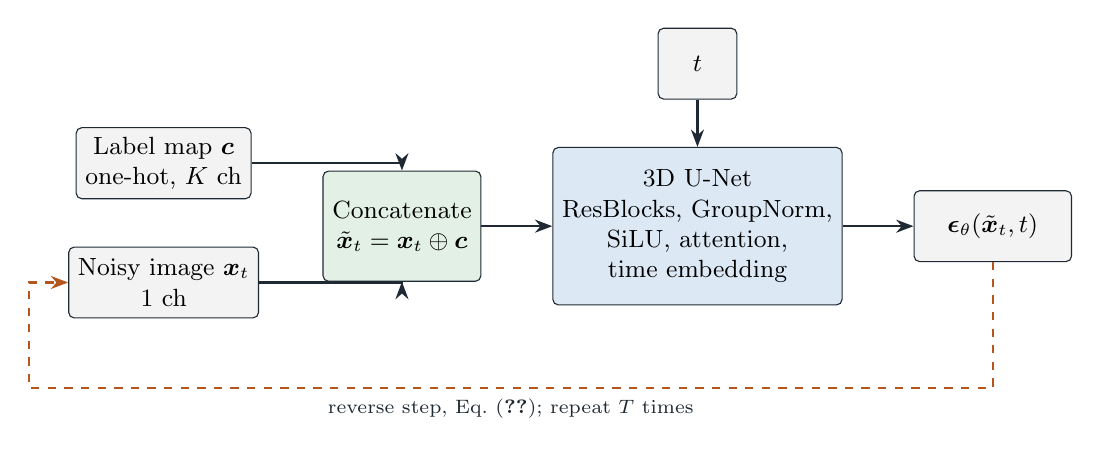
\begin{tikzpicture}[node distance=6mm and 9mm]
\node[blkE] (lab) {Label map $\bm c$\\one-hot, $K$ ch};
\node[blkE, below=of lab] (xt) {Noisy image $\x_t$\\1 ch};
\node[blkC, right=of lab, yshift=-8mm, minimum height=14mm] (cat) {Concatenate\\$\tilde\x_t=\x_t\oplus\bm c$};
\node[blkA, right=of cat, minimum height=20mm, minimum width=34mm] (U) {3D U-Net\\ResBlocks, GroupNorm,\\SiLU, attention,\\time embedding};
\node[blkE, right=of U] (e) {$\eps_\theta(\tilde\x_t,t)$};
\node[blkE, above=6mm of U, minimum width=10mm] (t) {$t$};
\draw[arr] (lab) -| (cat); \draw[arr] (xt) -| (cat); \draw[arr] (cat)--(U); \draw[arr] (U)--(e); \draw[arr] (t)--(U);
\draw[darr] (e.south) |- ++(0,-16mm) -| node[lbl,pos=0.25,below]{reverse step, Eq.~\eqref{eq:mdd-rev}; repeat $T$ times} ($(xt.west)+(-5mm,0)$) -- (xt.west);
\end{tikzpicture}
\end{adjustbox}
\caption{Med-DDPM (redrawn). The label map is concatenated to the noisy image at every step.}
\end{figure}


\textbf{Details.} 3D U-Net with ResBlocks, GroupNorm, SiLU, attention and a time embedding.

\subsection*{A.4 Maths and loss}
\textbf{Input.} Stick the one-hot label map $\bm c$ to the noisy image: $\tilde\x_t = \x_t\oplus\bm c$.

\textbf{Noise and generation} as in Chapter~\ref{ch:lefusion}, with $\eps_\theta(\tilde\x_t,t)$:
\begin{equation}\label{eq:mdd-rev}
\x_{t-1}=\frac{1}{\sqrt{\alpha_t}}\Big(\x_t-\frac{1-\alpha_t}{\sqrt{1-\abar_t}}\,\eps_\theta(\tilde\x_t,t)\Big)+\sigma_t\,\bm n .
\end{equation}
\textbf{Loss} (mean absolute error on the noise):
\begin{equation}
\Loss_{\text{MAE}}=\frac{1}{n}\sum_{i=1}^{n}\big|\epsilon_i-\epsilon_{\theta,i}(\tilde\x_t,t)\big|,\qquad n=D\cdot H\cdot W .
\end{equation}
Settings: $T=250$, cosine schedule; Adam, learning rate $10^{-5}$ (50k iterations) then $10^{-6}$ (50k); batch 1; EMA 0.995.

\subsection*{A.5 Input and output}
\begin{center}
\small
\begin{tabularx}{\linewidth}{lX}
\toprule
\textbf{Input} & one-hot label map + noise \\
\textbf{Output} & full 3D image that matches the labels \\
\textbf{Loss} & $\Loss_{\text{MAE}}$ \\
\bottomrule
\end{tabularx}
\end{center}

\subsection*{A.6 Results in the paper}
1{,}292 training brain MRIs at $128^3$. Tumour segmentation Dice: real 0.6531; synthetic only 0.6207; real + synthetic 0.6675.

\section{Part B -- Our dataset}

\subsection*{B.1 What data this method needs}
$\approx$1{,}000 region crops ($128^3$ at 0.45\,mm $\approx$ 58\,mm cube, around the circle of Willis) with 4-class label maps: background/soft tissue, vessel, aneurysm, bone (Common Step 3).

\subsection*{B.2 How we train it}
\textbf{Train from scratch, all layers.} No pretrained model of this kind exists for CTA. LoRA is not relevant.

\subsection*{B.3 Step-by-step pipeline}
\begin{enumerate}
  \item Run Common Steps 1--5. Cut one $128^3$ crop per case.
  \item Make the 4-class label map for each crop.
  \item \textbf{Train} with $\Loss_{\text{MAE}}$, $T=250$, batch 1--2, about 100k iterations. Use mixed precision and gradient checkpointing to save memory.
  \item \textbf{Make new label maps}: take a real one, remove the aneurysm, add a new one at a branch (Step 6) with a shape from the library.
  \item \textbf{Generate} the full crop. Use it as a training sample, or put it back with a wide soft edge.
\end{enumerate}

\subsection*{B.4 Compute}
40--80\,GB GPU for $128^3$; training 4--10 days (estimate); a few minutes per crop.

\subsection*{B.5 How to check it worked}
Check that generated vessels follow the label map; compare HU of tissue, vessels and aneurysm with real crops; visual check; Chapter~\ref{ch:eval}.

\subsection*{B.6 Risks}
\begin{caution}
The model copies the label map. Our vessel labels come from simple thresholds, so their mistakes become image mistakes. Every voxel is generated, so any odd texture can become a shortcut for the segmenter. Not possible in Case A (99 crops is too few).
\end{caution}

\subsection*{B.7 Rank for our dataset}
\begin{verdict}{Rank 6 of 8}
\begin{tabular}{ll}
Small-lesion detail & \stars{4}\\
Fits our data size & \stars{2} (from scratch)\\
Compute (5 = cheap) & \stars{2}\\
Code available & \stars{4}\\
Mask is exact & \stars{4}\\
Effort (5 = easy) & \stars{3}\\
\end{tabular}

\smallskip
Simple design and full control of vessels and aneurysm. Held back by training from scratch and rough vessel labels.
\end{verdict}

% =================== METHOD 7: MedGen3D ===================
\chapter{Method 7 -- MedGen3D}\label{ch:medgen3d}

\section{Part A -- The paper}

\subsection*{A.1 Idea}
\begin{idea}
First a diffusion model makes a new 3D label map, a few slices at a time. Then a video-style GAN turns the labels into an image, and three 2D diffusion models (one per direction) polish it.
\end{idea}
\textbf{Paper.} K.~Han, Y.~Xiong, C.~You, \emph{et al.}, ``MedGen3D: A Deep Generative Framework for Paired 3D Image and Mask Generation'', MICCAI 2023~\cite{han2023medgen3d}. Code: not given in the paper. Special point: it creates \emph{new anatomy}, not only new texture.

\subsection*{A.2 Basics you need: classifier-free guidance}
Train one model that sometimes gets the condition and sometimes not ($\varnothing$). At generation, push toward the condition with strength $s$~\cite{ho2022cfg}:
\begin{equation}
\hat\eps_\theta(X_t\mid\bm c)=\eps_\theta(X_t\mid\varnothing)+s\,\big(\eps_\theta(X_t\mid\bm c)-\eps_\theta(X_t\mid\varnothing)\big).
\end{equation}

\subsection*{A.3 Architecture}
\begin{figure}[H]
\centering
\begin{adjustbox}{max width=\linewidth}
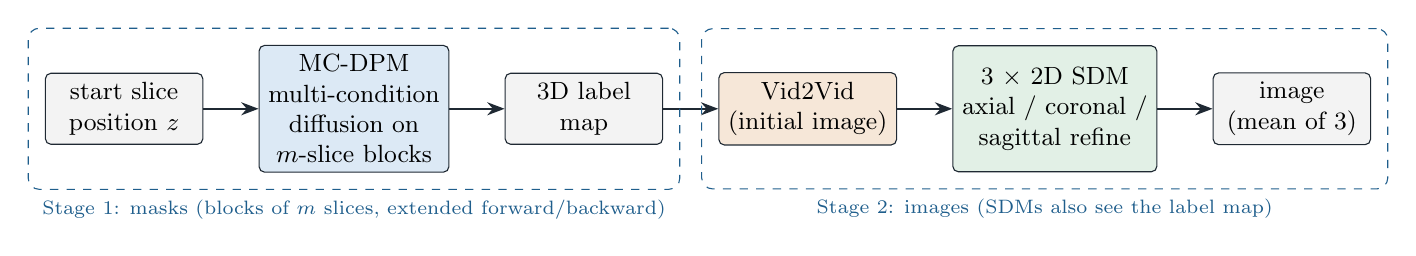
\begin{tikzpicture}[node distance=6mm and 7mm]
\node[blkE] (z) {start slice\\position $z$};
\node[blkA, right=of z, minimum height=16mm] (mc) {MC-DPM\\multi-condition\\diffusion on\\$m$-slice blocks};
\node[blkE, right=of mc] (mask) {3D label\\map};
\node[blkB, right=of mask] (v2v) {Vid2Vid\\(initial image)};
\node[blkC, right=of v2v, minimum height=16mm] (sdm) {3 $\times$ 2D SDM\\axial / coronal /\\sagittal refine};
\node[blkE, right=of sdm] (img) {image\\(mean of 3)};
\draw[arr] (z)--(mc); \draw[arr] (mc)--(mask); \draw[arr] (mask)--(v2v); \draw[arr] (v2v)--(sdm); \draw[arr] (sdm)--(img);
\node[grp, fit=(z)(mc)(mask), label={[lbl,text=acc]below:Stage 1: masks (blocks of $m$ slices, extended forward/backward)}] {};
\node[grp, fit=(v2v)(sdm)(img), label={[lbl,text=acc]below:Stage 2: images (SDMs also see the label map)}] {};
\end{tikzpicture}
\end{adjustbox}
\caption{MedGen3D (redrawn). Stage 1 builds a 3D mask from slice blocks; Stage 2 paints it.}
\end{figure}


\subsection*{A.4 Maths and loss}
\textbf{Stage 1: masks (MC-DPM).} Cut the label volume into blocks of $m=6$ slices. A block is made either from nothing, or from the first $n$ slices, or from the last $n$ slices (picked at random in training), plus its position $z/D$. With $X^P$ = slices to predict and $X^C$ = given slices (paper Eq.~4):
\begin{equation}
\Loss(\theta)=\E_{X_0,\eps,p^C,z,t}\Big[\norm{\eps-\eps_\theta\big(X_t^P,X^C,z,t\big)}^2\Big].
\end{equation}
To make a full volume: make one block at a random place, then grow it forward and backward, $(m-n)$ slices at a time.

\textbf{Stage 2: images.} Vid2Vid (a video GAN) turns the slice sequence of labels into images, keeping neighbouring slices consistent. Then three 2D diffusion models (axial, coronal, sagittal) refine it with 10 small steps, and the three results are averaged.

\subsection*{A.5 Input and output}
\begin{center}
\small
\begin{tabularx}{\linewidth}{lX}
\toprule
\textbf{Stage 1} & noise + position (+ known slices) $\rightarrow$ new label block \\
\textbf{Stage 2} & label map $\rightarrow$ image \\
\textbf{Output} & matched pair: image + label map \\
\bottomrule
\end{tabularx}
\end{center}

\subsection*{A.6 Results in the paper}
Chest CT (SegTHOR), Swin-UNETR Dice: real 0.878; synthetic only 0.854; real + synthetic 0.886; pre-train on synthetic then fine-tune 0.899. Trained on small sets (30 CT, 50 MRI).

\section{Part B -- Our dataset}

\subsection*{B.1 What data this method needs}
$\approx$1{,}000 region crops ($\approx$128 slices) with label maps: vessel, aneurysm, bone, background. Masks without scans cannot train Stage 1, because the vessels around the aneurysm are missing.

\subsection*{B.2 How we train it}
\textbf{Train all five networks from scratch} (MC-DPM, Vid2Vid, three 2D diffusion models). No released models. LoRA is not relevant.

\subsection*{B.3 Step-by-step pipeline}
\begin{enumerate}
  \item Run Common Steps 1--4; make label maps for region crops.
  \item Train MC-DPM on label blocks ($m=6$, $n=2$--$4$).
  \item Train Vid2Vid on label-slice $\rightarrow$ CT-slice sequences.
  \item Train the three 2D diffusion models.
  \item Generate new label maps, then images. Check that new aneurysms sit on vessels.
\end{enumerate}

\subsection*{B.4 Compute}
1--2 GPUs of 40\,GB; 1--2 weeks for all five networks (estimate).

\subsection*{B.5 How to check it worked}
Check new label maps first (vessels connected? aneurysms on vessels?). Look for seams between slice blocks. Then Chapter~\ref{ch:eval}.

\subsection*{B.6 Risks}
\begin{caution}
Five networks, no official code, and a 2.5D design. Round objects that cross many slices, like aneurysms, are exactly where 2.5D methods show seams. Highest effort of all eight. Not possible in Case A.
\end{caution}

\subsection*{B.7 Rank for our dataset}
\begin{verdict}{Rank 7 of 8}
\begin{tabular}{ll}
Small-lesion detail & \stars{3}\\
Fits our data size & \stars{3}\\
Compute (5 = cheap) & \stars{2}\\
Code available & \stars{1}\\
Mask is exact & \stars{4}\\
Effort (5 = easy) & \stars{1}\\
\end{tabular}

\smallskip
Nice idea (new anatomy), but too complex here. LeFusion's DiffMask already gives new shapes more simply.
\end{verdict}

% =================== METHOD 8: brainSPADE ===================
\chapter{Method 8 -- brainSPADE}\label{ch:spade}

\section{Part A -- The paper}

\subsection*{A.1 Idea}
\begin{idea}
Two models. A latent diffusion model invents new label maps. A SPADE GAN paints any label map as an image, in a chosen style. Together they make fully synthetic image + label pairs.
\end{idea}
\textbf{Paper.} V.~Fernandez, W.~H.~L.~Pinaya, P.~Borges, \emph{et al.}, ``Can Segmentation Models Be Trained with Fully Synthetically Generated Data?'', SASHIMI (MICCAI workshop) 2022~\cite{fernandez2022brainspade}. Code: not released. Works on 2D slices ($192\times256$).

\subsection*{A.2 Basics you need: VAE and SPADE}
\textbf{VAE.} An autoencoder whose code is pushed to look like standard Gaussian noise, using a KL term $D_{\text{KL}}\big(\enc(\bm l)\,\Vert\,\N(\bm 0,\I)\big)$. Then new codes can be sampled.

\textbf{SPADE normalisation}~\cite{park2019spade}. Inside the generator, every normalisation layer is steered by the label map $\bm l$. For feature $h$ at channel $c$ and position $(y,x)$:
\begin{equation}
h'=\gamma_{c,y,x}(\bm l)\cdot\frac{h_{c,y,x}-\mu_c}{\sigma_c}+\beta_{c,y,x}(\bm l).
\end{equation}
$\gamma$ and $\beta$ come from small convolutions on $\bm l$, so the labels are present in every layer.

\subsection*{A.3 Architecture}
\begin{figure}[H]
\centering
\begin{adjustbox}{max width=\linewidth}
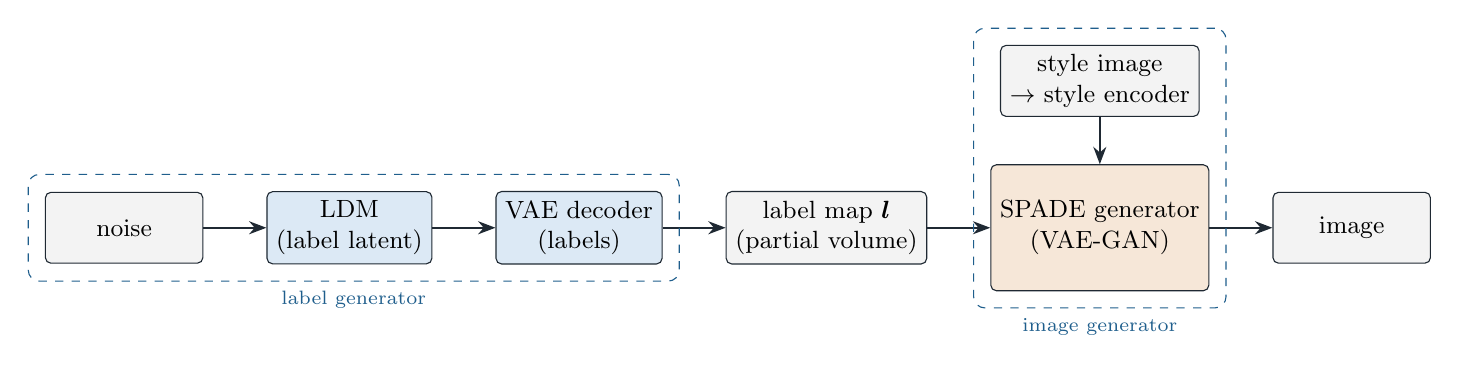
\begin{tikzpicture}[node distance=6mm and 8mm]
\node[blkE] (n) {noise};
\node[blkA, right=of n] (ldm) {LDM\\(label latent)};
\node[blkA, right=of ldm] (vd) {VAE decoder\\(labels)};
\node[blkE, right=of vd] (l) {label map $\bm l$\\(partial volume)};
\node[blkB, right=of l, minimum height=16mm] (sp) {SPADE generator\\(VAE-GAN)};
\node[blkE, right=of sp] (img) {image};
\node[blkE, above=6mm of sp] (sty) {style image\\$\rightarrow$ style encoder};
\draw[arr] (n)--(ldm); \draw[arr] (ldm)--(vd); \draw[arr] (vd)--(l); \draw[arr] (l)--(sp); \draw[arr] (sp)--(img); \draw[arr] (sty)--(sp);
\node[grp, fit=(n)(ldm)(vd), label={[lbl,text=acc]below:label generator}] {};
\node[grp, fit=(sp)(sty), label={[lbl,text=acc]below:image generator}] {};
\end{tikzpicture}
\end{adjustbox}
\caption{brainSPADE (redrawn). Labels are generated first, then painted by SPADE.}
\end{figure}


\subsection*{A.4 Maths and loss}
\textbf{Label generator.} VAE (code $48\times64\times3$) + latent diffusion (1000 steps, $L_1$ loss on noise). VAE loss:
\begin{equation}
\Loss_{\text{VAE}}=D_{\text{KL}}\big(\enc(\bm l)\Vert\N(\bm 0,\I)\big)+\Loss_{\text{perc}}(\bm l,\hat{\bm l})+\Loss_{\text{adv}}+\norm{\hat{\bm l}-\bm l}_1 .
\end{equation}
Labels are soft maps (partial volume). Separate models for healthy and tumour labels.

\textbf{Image generator} (paper weights):
\begin{equation}
\Loss_G=1.0\,\Loss_{\text{adv}}^{\text{hinge}}+0.25\,\Loss_{\text{VGG}}+0.05\,\Loss_{\text{FM}}+0.001\,\Loss_{\text{KL}}+1.0\,\Loss_{\text{contrastive}}+\Loss_{\text{mod,dat}} ,
\end{equation}
with a style-contrastive term $\Loss_{\text{contrastive}}=\operatorname{cosim}\big(E_s(i),E_s(T(i))\big)$ and small classifiers for modality and dataset.

\subsection*{A.5 Input and output}
\begin{center}
\small
\begin{tabularx}{\linewidth}{lX}
\toprule
\textbf{Label generator} & noise $\rightarrow$ 2D label map \\
\textbf{Image generator} & label map + style image $\rightarrow$ 2D image \\
\textbf{Output} & 2D image + label pair \\
\bottomrule
\end{tabularx}
\end{center}

\subsection*{A.6 Results in the paper}
Tumour Dice (2D nnU-Net): real 0.813; synthetic only 0.760; real + synthetic 0.876. Image generator trained about 2 weeks on one Quadro RTX 8000.

\section{Part B -- Our dataset}

\subsection*{B.1 What data this method needs}
Axial 2D slices from region crops, with soft label maps (vessel, aneurysm, bone, background).

\subsection*{B.2 How we train it}
\textbf{Train from scratch} (label VAE, latent diffusion, SPADE GAN). No released models. LoRA is not relevant.

\subsection*{B.3 Step-by-step pipeline}
\begin{enumerate}
  \item Run Common Steps 1--4; cut axial slices; make soft labels by blurring the binary labels.
  \item Train the label VAE + latent diffusion (a separate one for slices with aneurysm).
  \item Train SPADE on (label, CT) slice pairs; style image = another slice of the same scan.
  \item Generate 2D pairs. Stacking them into 3D will not be consistent.
\end{enumerate}

\subsection*{B.4 Compute}
One 24\,GB GPU; 1--2 weeks (estimate). Generation is fast.

\subsection*{B.5 How to check it worked}
Look at neighbouring generated slices: the aneurysm should not jump or change shape. Then Chapter~\ref{ch:eval} (2D version).

\subsection*{B.6 Risks}
\begin{caution}
An aneurysm crosses 10--25 slices. Making each slice separately breaks its 3D shape. A 3D SPADE would fix this, but that is a new research project.
\end{caution}

\subsection*{B.7 Rank for our dataset}
\begin{verdict}{Rank 8 of 8}
\begin{tabular}{ll}
Small-lesion detail & \stars{2}\\
Fits our data size & \stars{3}\\
Compute (5 = cheap) & \stars{4}\\
Code available & \stars{1}\\
Mask is exact & \stars{3}\\
Effort (5 = easy) & \stars{2}\\
\end{tabular}

\smallskip
Shows the idea of fully synthetic pairs well, but only useful here for 2D tests.
\end{verdict}

% =================== BASELINE ===================
\chapter{Simple baseline (no AI)}\label{ch:baseline}

\begin{idea}
Draw the aneurysm with simple rules: take a mask shape, fill it with vessel-like brightness, blur it like the scanner does, add matching noise.
\end{idea}
Similar ideas helped in published work: VaMos on MRA~\cite{rochette2024vamos} (sensitivity 75.6\% $\rightarrow$ 89.0\%, but false positives per scan 0.22 $\rightarrow$ 0.40) and synthetic liver tumours in CT~\cite{hu2023labelfree}.

\textbf{Formula.} For a placed mask $\m$, with parent-vessel brightness $\mu_v$ and spread $\sigma_v$ measured nearby:
\begin{equation}
\x^{\text{new}}=(1-w)\had\x+w\had\big(\mu_a+\sigma_v\cdot\text{blur}(\bm n)\big),\qquad w=\text{blur}_{0.5\text{--}0.8\,\text{mm}}(\m),\quad \bm n\sim\N(\bm 0,\I),
\end{equation}
with $\mu_a$ a bit below or equal to $\mu_v$ (85--105\%).

\textbf{Why keep it.} It takes hours to build. If a generative method cannot beat it on real test data, the extra cost is not worth it.

% =================== EVALUATION ===================
\chapter{One fair test for all methods}\label{ch:eval}

Every method is tested the same way, on \textbf{real} data only.

\section*{1. Does it look real?}
\addcontentsline{toc}{section}{1. Does it look real?}
\begin{itemize}
  \item \textbf{Fr\'echet distance} between real and synthetic aneurysm patches, using features $\phi$ from a 3D medical network (e.g.\ MedicalNet~\cite{chen2019med3d}):
  \begin{equation}
  \text{FD}=\norm{\bm\mu_r-\bm\mu_s}_2^2+\operatorname{Tr}\Big(\Sigma_r+\Sigma_s-2(\Sigma_r\Sigma_s)^{1/2}\Big).
  \end{equation}
  Lower is better.
  \item \textbf{Brightness inside the aneurysm}: mean, spread and histogram vs.\ real.
  \item \textbf{Shape}: volume and roundness $\Psi=\pi^{1/3}(6V)^{2/3}/A$ vs.\ real.
  \item \textbf{Human test}: 100 real + 100 synthetic patches, mixed; can a reader tell them apart? 50\% correct = cannot tell.
\end{itemize}

\section*{2. Is it copying?}
\addcontentsline{toc}{section}{2. Is it copying?}
For each synthetic patch, find the closest training patch:
\begin{equation}
d(\hat\x)=\min_{\x\in\text{train}}\ 1-\cos\big(\phi(\hat\x),\phi(\x)\big).
\end{equation}
If many synthetic patches are closer to a training patch than two different real patches usually are, the model is copying.

\section*{3. Does it help? (the real test)}
\addcontentsline{toc}{section}{3. Does it help? (the real test)}
Train nnU-Net~\cite{isensee2021nnunet} (3d\_fullres, same settings, 3 seeds) on:
\begin{center}
\small
\begin{tabular}{ll}
\toprule
\textbf{Run} & \textbf{Training data} \\
\midrule
R & real only \\
R + B & real + simple baseline \\
R + S & real + synthetic from one method (synthetic:real = 0.5, 1, 2) \\
S & synthetic only (just to see) \\
\bottomrule
\end{tabular}
\end{center}
\textbf{Measure on the real test set:}
\begin{itemize}
  \item Dice on cases with aneurysms;
  \item found aneurysms (sensitivity), split by size: $<3$, 3--5, 5--10, $>10$\,mm;
  \item false alarms per scan;
  \item on the 50 test scans without aneurysms: how many are correctly called ``no aneurysm'';
  \item 95\% confidence intervals by bootstrap (1{,}000 resamples).
\end{itemize}
\begin{caution}
Synthetic data often finds more aneurysms \emph{and} gives more false alarms. Always report both.
\end{caution}

% =================== LICENCE ===================
\chapter{Dataset licence}\label{ch:licence}

\textbf{Source.} Bo ZH, Qiao H, Tian C, \emph{et al.}, \emph{Patterns} 2(2):100197, 2021~\cite{bo2021}. 1{,}338 internal cases from six hospitals (1{,}489 aneurysms) and two outside test sets.

\textbf{Licence -- please confirm.} The \emph{article} is CC BY-NC-ND 4.0. The \emph{data} is reported to be for \textbf{non-commercial use}. We could not open the data website to read the exact terms. Read the terms that came with your download.

\textbf{Until confirmed:}
\begin{itemize}
  \item Use the data and all synthetic data from it for non-commercial research only.
  \item Do not share the original scans. Treat synthetic scans the same way (they are built on real scans).
  \item Cite Bo et al.\ (2021).
  \item Check model licences: MAISI code Apache-2.0, weights NVIDIA Open Model licence; check LeFusion, DiffTumor and Med-DDPM licence files.
  \item Name synthetic files \texttt{Syn\_...} and keep the log.
\end{itemize}

% =================== SUMMARY ===================
\chapter{Summary, ranking and roadmap}\label{ch:summary}

\section*{Final ranking (Case B, $\approx$1{,}338 scans)}
\addcontentsline{toc}{section}{Final ranking}
\begin{center}
\small
\begin{tabular}{clcccccc}
\toprule
\textbf{Rank} & \textbf{Method} & \textbf{Lesion} & \textbf{Data fit} & \textbf{Compute} & \textbf{Code} & \textbf{Mask} & \textbf{Effort} \\
\midrule
1 & LeFusion & 5 & 4 & 4 & 4 & 5 & 3 \\
2 & DiffTumor & 3 & 4 & 3 & 5 & 4 & 3 \\
3 & 3D cGAN (Jin) & 4 & 4 & 5 & 2 & 3 & 4 \\
4 & RePaint & 4 & 3 & 3 & 3 & 2 & 4 \\
5 & MAISI-v2 + ControlNet & 2 & 4 & 2 & 5 & 3 & 2 \\
6 & Med-DDPM & 4 & 2 & 2 & 4 & 4 & 3 \\
7 & MedGen3D & 3 & 3 & 2 & 1 & 4 & 1 \\
8 & brainSPADE & 2 & 3 & 4 & 1 & 3 & 2 \\
\bottomrule
\end{tabular}
\end{center}
1 = poor, 5 = best (for Compute and Effort, 5 = cheapest/easiest). The rank is a judgement, not a sum: \emph{lesion detail} and \emph{exact mask} matter most.

\section*{How each method is trained}
\addcontentsline{toc}{section}{How each method is trained}
\begin{center}
\small
\begin{tabularx}{\linewidth}{lXl}
\toprule
\textbf{Method} & \textbf{Scratch / fine-tune / frozen / LoRA} & \textbf{GPU (estimate)} \\
\midrule
LeFusion & from scratch (option: start from lung model, fine-tune all) & 24--40\,GB, 1--3 days \\
DiffTumor & AE fine-tune all, or from scratch with compression 2; diffusion from scratch & 40\,GB, 4--8 days \\
3D cGAN & from scratch & 16--24\,GB, $<$1 day \\
RePaint & diffusion from scratch; filling needs no training & 24\,GB, 1--3 days \\
MAISI-v2 & VAE + U-Net frozen; LoRA on U-Net; ControlNet trained & 40--80\,GB, 3--7 days \\
Med-DDPM & from scratch & 40--80\,GB, 4--10 days \\
MedGen3D & all five networks from scratch & 40\,GB, 1--2 weeks \\
brainSPADE & from scratch & 24\,GB, 1--2 weeks \\
\bottomrule
\end{tabularx}
\end{center}
A MacBook Air cannot train these. Use Kaggle, Colab Pro, or a rented cloud GPU. Upload patches ($\approx$3\,GB), not full scans ($\approx$180\,GB).

\section*{Main points}
\addcontentsline{toc}{section}{Main points}
\begin{enumerate}
  \item \textbf{Filling a mask in a real scan beats making whole scans} for tiny aneurysms.
  \item \textbf{Full resolution beats compressed codes} for 3--5\,mm lesions.
  \item \textbf{Where you put the aneurysm matters as much as the model.}
  \item \textbf{Masks without scans are useful} for the shape library and DiffMask.
  \item \textbf{99 scans is only for testing code.} Real training needs the full download.
  \item \textbf{Judge only on real test data}, and report found aneurysms \emph{and} false alarms.
\end{enumerate}

\section*{Roadmap}
\addcontentsline{toc}{section}{Roadmap}
\begin{center}
\small
\begin{tabularx}{\linewidth}{lXl}
\toprule
\textbf{Phase} & \textbf{Work} & \textbf{Result} \\
\midrule
0 & Download; Common Steps 1--5 (Chapter~\ref{ch:prep}) & patch dataset \\
1 & Simple baseline; nnU-Net runs R and R+B & reference numbers \\
2 & LeFusion + DiffMask; full test & first generative result \\
3 & 3D cGAN as fast comparison; DiffTumor if LeFusion struggles & comparison \\
4 & (Optional) MAISI-v2 + LoRA + ControlNet for regions & advanced \\
5 & Outside test (if external scans obtained) & generalisation \\
\bottomrule
\end{tabularx}
\end{center}

\begin{verdict}{Recommendation}
Do the common steps and the simple baseline first. Then build \textbf{LeFusion} on $64^3$ aneurysm patches, trained from scratch, with DiffMask for new shapes. Compare it with the 3D cGAN and the baseline using nnU-Net on real test data. Try MAISI-v2 only if region realism becomes the problem and big GPUs are available.
\end{verdict}

\cleardoublepage\phantomsection\addcontentsline{toc}{chapter}{References}
\renewcommand{\bibname}{References}

\begin{thebibliography}{99}\small
\bibitem{bo2021} Z.-H.~Bo, H.~Qiao, C.~Tian, \emph{et al.} Toward human intervention-free clinical diagnosis of intracranial aneurysm via deep neural network. \emph{Patterns}, 2(2):100197, 2021. doi:10.1016/j.patter.2020.100197.
\bibitem{zhang2025lefusion} H.~Zhang, Y.~Liu, J.~Yang, \emph{et al.} LeFusion: Controllable pathology synthesis via lesion-focused diffusion models. \emph{ICLR}, 2025. arXiv:2403.14066.
\bibitem{chen2024difftumor} Q.~Chen, X.~Chen, H.~Song, \emph{et al.} Towards generalizable tumor synthesis. \emph{CVPR}, 2024. arXiv:2402.19470.
\bibitem{jin2018cgan} D.~Jin, Z.~Xu, Y.~Tang, \emph{et al.} CT-realistic lung nodule simulation from 3D conditional generative adversarial networks for robust lung segmentation. \emph{MICCAI}, 2018. arXiv:1806.04051.
\bibitem{lugmayr2022repaint} A.~Lugmayr, M.~Danelljan, A.~Romero, \emph{et al.} RePaint: Inpainting using denoising diffusion probabilistic models. \emph{CVPR}, 2022. arXiv:2201.09865.
\bibitem{guo2025maisi} P.~Guo, C.~Zhao, D.~Yang, \emph{et al.} MAISI: Medical AI for synthetic imaging. \emph{WACV}, 2025. arXiv:2409.11169.
\bibitem{zhao2025maisiv2} C.~Zhao, P.~Guo, D.~Yang, \emph{et al.} MAISI-v2: Accelerated 3D high-resolution medical image synthesis with rectified flow and region-specific contrastive loss. arXiv:2508.05772, 2025.
\bibitem{dorjsembe2024medddpm} Z.~Dorjsembe, H.-K.~Pao, S.~Odonchimed, \emph{et al.} Conditional diffusion models for semantic 3D brain MRI synthesis. \emph{IEEE J.\ Biomed.\ Health Inform.}, 2024. doi:10.1109/JBHI.2024.3385504.
\bibitem{han2023medgen3d} K.~Han, Y.~Xiong, C.~You, \emph{et al.} MedGen3D: A deep generative framework for paired 3D image and mask generation. \emph{MICCAI}, 2023. arXiv:2304.04106.
\bibitem{fernandez2022brainspade} V.~Fernandez, W.~H.~L.~Pinaya, P.~Borges, \emph{et al.} Can segmentation models be trained with fully synthetically generated data? \emph{SASHIMI (MICCAI workshop)}, 2022. arXiv:2209.08256.
\bibitem{rochette2024vamos} VaMos authors (Universit\'e de Nantes). A vascular synthetic model for improved aneurysm segmentation and detection via deep neural networks. arXiv:2403.18734, 2024.
\bibitem{hu2023labelfree} Q.~Hu, Y.~Chen, J.~Xiao, \emph{et al.} Label-free liver tumor segmentation. \emph{CVPR}, 2023. arXiv:2303.14869.
\bibitem{ho2020ddpm} J.~Ho, A.~Jain, P.~Abbeel. Denoising diffusion probabilistic models. \emph{NeurIPS}, 2020.
\bibitem{nichol2021} A.~Nichol, P.~Dhariwal. Improved denoising diffusion probabilistic models. \emph{ICML}, 2021.
\bibitem{song2021ddim} J.~Song, C.~Meng, S.~Ermon. Denoising diffusion implicit models. \emph{ICLR}, 2021.
\bibitem{rombach2022ldm} R.~Rombach, A.~Blattmann, D.~Lorenz, P.~Esser, B.~Ommer. High-resolution image synthesis with latent diffusion models. \emph{CVPR}, 2022.
\bibitem{esser2021vqgan} P.~Esser, R.~Rombach, B.~Ommer. Taming transformers for high-resolution image synthesis. \emph{CVPR}, 2021.
\bibitem{ho2022cfg} J.~Ho, T.~Salimans. Classifier-free diffusion guidance. arXiv:2207.12598, 2022.
\bibitem{liu2023rf} X.~Liu, C.~Gong, Q.~Liu. Flow straight and fast: Learning to generate and transfer data with rectified flow. \emph{ICLR}, 2023.
\bibitem{goodfellow2014gan} I.~Goodfellow \emph{et al.} Generative adversarial nets. \emph{NeurIPS}, 2014.
\bibitem{isola2017pix2pix} P.~Isola, J.-Y.~Zhu, T.~Zhou, A.~A.~Efros. Image-to-image translation with conditional adversarial networks. \emph{CVPR}, 2017.
\bibitem{zhang2023controlnet} L.~Zhang, A.~Rao, M.~Agrawala. Adding conditional control to text-to-image diffusion models. \emph{ICCV}, 2023.
\bibitem{hu2022lora} E.~J.~Hu \emph{et al.} LoRA: Low-rank adaptation of large language models. \emph{ICLR}, 2022.
\bibitem{park2019spade} T.~Park, M.-Y.~Liu, T.-C.~Wang, J.-Y.~Zhu. Semantic image synthesis with spatially-adaptive normalization. \emph{CVPR}, 2019.
\bibitem{frangi1998} A.~F.~Frangi, W.~J.~Niessen, K.~L.~Vincken, M.~A.~Viergever. Multiscale vessel enhancement filtering. \emph{MICCAI}, 1998.
\bibitem{chen2019med3d} S.~Chen, K.~Ma, Y.~Zheng. Med3D: Transfer learning for 3D medical image analysis. arXiv:1904.00625, 2019.
\bibitem{isensee2021nnunet} F.~Isensee, P.~F.~Jaeger, S.~A.~A.~Kohl, J.~Petersen, K.~H.~Maier-Hein. nnU-Net: a self-configuring method for deep learning-based biomedical image segmentation. \emph{Nature Methods}, 18:203--211, 2021.
\end{thebibliography}

\end{document}
